% Training Data Thresholds for Cost-Effective Korean Sentiment Analysis
% Build with XeLaTeX (Korean text via kotex): latexmk -xelatex main.tex   (or: tectonic main.tex)
% Tables (tables/), figures (figures/) and numbers (generated/numbers.tex) are
% auto-generated by source/scripts/06_analyze.sh -- edit the prose, not those files.
\documentclass[11pt,a4paper]{article}
\usepackage[margin=2.3cm]{geometry}
\usepackage{kotex}                                   % Hangul under XeLaTeX
\setmainhangulfont{UnBatang}[Extension=.ttf]         % ships with TeX Live (unfonts-core)
\setsanshangulfont{UnDotum}[Extension=.ttf]
\setmonohangulfont{UnDotum}[Extension=.ttf]
\usepackage{amsmath,amssymb}
\usepackage{graphicx}
\usepackage{booktabs,multirow,adjustbox,array}
\usepackage{xcolor}
\usepackage{caption,subcaption}
\usepackage{tikz}
\usetikzlibrary{arrows.meta,positioning,fit,calc}
\usepackage[numbers,sort&compress]{natbib}
\usepackage{microtype}
\usepackage[hidelinks]{hyperref}
\usepackage[capitalise,noabbrev]{cleveref}

\captionsetup{font=small,labelfont=bf}
\newcommand{\TBD}[1]{\textcolor{red}{\textbf{[TBD:\,#1]}}}
\newcommand{\pmnote}{Values are mean\,$\pm$\,standard deviation over \nSeeds{} seeds (sample standard deviation, ddof\,=\,1).}
% AUTO-GENERATED by ksent.analysis.make_numbers (do not edit by hand).
% Every number cited in the report/slides comes from these macros.

\newcommand{\nSeeds}{5}  % experiment seeds
\newcommand{\seedList}{13, 42, 87, 2024, 31337}  % seed values
\newcommand{\nFinalFits}{675}  % planned final fits
\newcommand{\nTuningFits}{270}  % planned tuning fits
\newcommand{\nThreads}{8}  % CPU threads
\newcommand{\crossoverMargin}{1.0}  % crossover margin (macro-F1 points)
\newcommand{\dataSeed}{2026}  % split seed
\newcommand{\cpuModel}{Apple M4}  % CPU model
\newcommand{\gpuModel}{Apple M4 GPU (MPS)}  % GPU / accelerator model
\newcommand{\trainDevice}{\TBD{trainDevice}}  % neural training device(s) of the reported runs
\newcommand{\accelDevice}{\TBD{accelDevice}}  % accelerator used for neural latency
\newcommand{\precisionUsed}{\TBD{precisionUsed}}  % numeric precision of reported runs
\newcommand{\mambaBackend}{\TBD{mambaBackend}}  % Mamba backend of reported runs
\newcommand{\hardwareNote}{all results from one machine}  % hardware consistency
\newcommand{\nRunsDone}{\TBD{nRunsDone}}  % successful main runs
\newcommand{\nAblationRunsDone}{\TBD{nAblationRunsDone}}  % successful ablation-only runs
\newcommand{\nAblationFits}{120}  % planned new ablation fits
\newcommand{\maxSeqLenKiwi}{72}  % max sequence length (kiwi)
\newcommand{\maxSeqLenWhitespace}{32}  % max sequence length (whitespace)
\newcommand{\maxSeqLenChar}{96}  % max sequence length (char)
\newcommand{\totalTuningHours}{\TBD{totalTuningHours}}  % total tuning fit time (h)
\newcommand{\totalSweepHours}{\TBD{totalSweepHours}}  % total wall time of final runs (h)
\newcommand{\nRawNSMC}{200{,}000}  % NSMC raw reviews
\newcommand{\nCleanNSMC}{193{,}909}  % NSMC reviews after cleaning
\newcommand{\nKiwiEmptyNSMC}{0}  % NSMC reviews dropped for zero Kiwi tokens
\newcommand{\nRatingThreeNSMC}{0}  % NSMC rating-3 reviews dropped
\newcommand{\symbolShareNSMC}{10.9\%}  % NSMC reviews containing kk/yu/h jamo or emoji
\newcommand{\truncKiwiNSMC}{2.5\%}  % NSMC train-pool reviews truncated (Kiwi)
\newcommand{\oovSmallNSMC}{20.5\%}  % NSMC test OOV token rate (Kiwi vocab) at n=500
\newcommand{\oovLargeNSMC}{5.9\%}  % NSMC test OOV token rate (Kiwi vocab) at n=8000
\newcommand{\ablationTfidfNSMC}{\TBD{ablationTfidfNSMC}}  % ablation TF-IDF method
\newcommand{\ablationNeuralNSMC}{\TBD{ablationNeuralNSMC}}  % ablation neural method
\newcommand{\ablationGapSmallNSMC}{\TBD{ablationGapSmallNSMC}}  % gap with each family's best tokenizer at n=500
\newcommand{\ablationGapLargeNSMC}{\TBD{ablationGapLargeNSMC}}  % gap with each family's best tokenizer at n=8000
\newcommand{\bestTokenizerTfidfNSMC}{\TBD{bestTokenizerTfidfNSMC}}  % best TF-IDF tokenizer (validation) at n=8000
\newcommand{\bestTokenizerNeuralNSMC}{\TBD{bestTokenizerNeuralNSMC}}  % best neural tokenizer (validation) at n=8000
\newcommand{\ablationHoldsNSMC}{\TBD{ablationHoldsNSMC}}  % does the main conclusion hold with the best tokenizers
\newcommand{\crossoverNSMC}{\TBD{crossoverNSMC}}  % NSMC crossover threshold (val-selected winners)
\newcommand{\crossoverTestSelNSMC}{\TBD{crossoverTestSelNSMC}}  % NSMC threshold with test-selected winners (sensitivity)
\newcommand{\evalSizeNSMC}{\TBD{evalSizeNSMC}}  % size used for the Pareto check
\newcommand{\bestTfidfNSMC}{\TBD{bestTfidfNSMC}}  % best TF-IDF method at eval size
\newcommand{\bestNeuralNSMC}{\TBD{bestNeuralNSMC}}  % best neural method at eval size
\newcommand{\gapNSMC}{\TBD{gapNSMC}}  % neural - TF-IDF test macro-F1 gap at eval size (points)
\newcommand{\paretoNSMC}{\TBD{paretoNSMC}}  % is the neural winner Pareto-efficient vs the TF-IDF winner
\newcommand{\latencyRatioNSMC}{\TBD{latencyRatioNSMC}}  % neural / TF-IDF latency ratio
\newcommand{\fitRatioNSMC}{\TBD{fitRatioNSMC}}  % neural / TF-IDF fit ratio
\newcommand{\ramRatioNSMC}{\TBD{ramRatioNSMC}}  % neural / TF-IDF ram ratio
\newcommand{\tfidfLatencyNSMC}{\TBD{tfidfLatencyNSMC}}  % TF-IDF winner CPU e2e ms
\newcommand{\neuralLatencyNSMC}{\TBD{neuralLatencyNSMC}}  % neural winner CPU e2e ms
\newcommand{\bestMethodNSMC}{\TBD{bestMethodNSMC}}  % best method by test macro-F1 at n=8000
\newcommand{\macroFOneBestNSMC}{\TBD{macroFOneBestNSMC}}  % its test macro-F1 (x100) at n=8000
\newcommand{\bestEightKTfidfNSMC}{\TBD{bestEightKTfidfNSMC}}  % val-selected best tfidf at n=8000
\newcommand{\macroFOneEightKTfidfNSMC}{\TBD{macroFOneEightKTfidfNSMC}}  % its test macro-F1 (x100) at n=8000
\newcommand{\bestEightKNeuralNSMC}{\TBD{bestEightKNeuralNSMC}}  % val-selected best neural at n=8000
\newcommand{\macroFOneEightKNeuralNSMC}{\TBD{macroFOneEightKNeuralNSMC}}  % its test macro-F1 (x100) at n=8000
\newcommand{\mambaFOneNSMC}{\TBD{mambaFOneNSMC}}  % Mamba test macro-F1 at n=8000
\newcommand{\gainFirstNSMC}{\TBD{gainFirstNSMC}}  % best method's macro-F1 gain 500->1000 (points)
\newcommand{\gainLastNSMC}{\TBD{gainLastNSMC}}  % best method's macro-F1 gain 4000->8000 (points)
\newcommand{\nRawShopping}{200{,}000}  % Shopping raw reviews
\newcommand{\nCleanShopping}{199{,}881}  % Shopping reviews after cleaning
\newcommand{\nKiwiEmptyShopping}{0}  % Shopping reviews dropped for zero Kiwi tokens
\newcommand{\nRatingThreeShopping}{0}  % Shopping rating-3 reviews dropped
\newcommand{\symbolShareShopping}{13.1\%}  % Shopping reviews containing kk/yu/h jamo or emoji
\newcommand{\truncKiwiShopping}{1.2\%}  % Shopping train-pool reviews truncated (Kiwi)
\newcommand{\oovSmallShopping}{16.6\%}  % Shopping test OOV token rate (Kiwi vocab) at n=500
\newcommand{\oovLargeShopping}{4.2\%}  % Shopping test OOV token rate (Kiwi vocab) at n=8000
\newcommand{\ablationTfidfShopping}{\TBD{ablationTfidfShopping}}  % ablation TF-IDF method
\newcommand{\ablationNeuralShopping}{\TBD{ablationNeuralShopping}}  % ablation neural method
\newcommand{\ablationGapSmallShopping}{\TBD{ablationGapSmallShopping}}  % gap with each family's best tokenizer at n=500
\newcommand{\ablationGapLargeShopping}{\TBD{ablationGapLargeShopping}}  % gap with each family's best tokenizer at n=8000
\newcommand{\bestTokenizerTfidfShopping}{\TBD{bestTokenizerTfidfShopping}}  % best TF-IDF tokenizer (validation) at n=8000
\newcommand{\bestTokenizerNeuralShopping}{\TBD{bestTokenizerNeuralShopping}}  % best neural tokenizer (validation) at n=8000
\newcommand{\ablationHoldsShopping}{\TBD{ablationHoldsShopping}}  % does the main conclusion hold with the best tokenizers
\newcommand{\crossoverShopping}{\TBD{crossoverShopping}}  % Shopping crossover threshold (val-selected winners)
\newcommand{\crossoverTestSelShopping}{\TBD{crossoverTestSelShopping}}  % Shopping threshold with test-selected winners (sensitivity)
\newcommand{\evalSizeShopping}{\TBD{evalSizeShopping}}  % size used for the Pareto check
\newcommand{\bestTfidfShopping}{\TBD{bestTfidfShopping}}  % best TF-IDF method at eval size
\newcommand{\bestNeuralShopping}{\TBD{bestNeuralShopping}}  % best neural method at eval size
\newcommand{\gapShopping}{\TBD{gapShopping}}  % neural - TF-IDF test macro-F1 gap at eval size (points)
\newcommand{\paretoShopping}{\TBD{paretoShopping}}  % is the neural winner Pareto-efficient vs the TF-IDF winner
\newcommand{\latencyRatioShopping}{\TBD{latencyRatioShopping}}  % neural / TF-IDF latency ratio
\newcommand{\fitRatioShopping}{\TBD{fitRatioShopping}}  % neural / TF-IDF fit ratio
\newcommand{\ramRatioShopping}{\TBD{ramRatioShopping}}  % neural / TF-IDF ram ratio
\newcommand{\tfidfLatencyShopping}{\TBD{tfidfLatencyShopping}}  % TF-IDF winner CPU e2e ms
\newcommand{\neuralLatencyShopping}{\TBD{neuralLatencyShopping}}  % neural winner CPU e2e ms
\newcommand{\bestMethodShopping}{\TBD{bestMethodShopping}}  % best method by test macro-F1 at n=8000
\newcommand{\macroFOneBestShopping}{\TBD{macroFOneBestShopping}}  % its test macro-F1 (x100) at n=8000
\newcommand{\bestEightKTfidfShopping}{\TBD{bestEightKTfidfShopping}}  % val-selected best tfidf at n=8000
\newcommand{\macroFOneEightKTfidfShopping}{\TBD{macroFOneEightKTfidfShopping}}  % its test macro-F1 (x100) at n=8000
\newcommand{\bestEightKNeuralShopping}{\TBD{bestEightKNeuralShopping}}  % val-selected best neural at n=8000
\newcommand{\macroFOneEightKNeuralShopping}{\TBD{macroFOneEightKNeuralShopping}}  % its test macro-F1 (x100) at n=8000
\newcommand{\mambaFOneShopping}{\TBD{mambaFOneShopping}}  % Mamba test macro-F1 at n=8000
\newcommand{\gainFirstShopping}{\TBD{gainFirstShopping}}  % best method's macro-F1 gain 500->1000 (points)
\newcommand{\gainLastShopping}{\TBD{gainLastShopping}}  % best method's macro-F1 gain 4000->8000 (points)
\newcommand{\nRawSteam}{100{,}000}  % Steam raw reviews
\newcommand{\nCleanSteam}{99{,}774}  % Steam reviews after cleaning
\newcommand{\nKiwiEmptySteam}{0}  % Steam reviews dropped for zero Kiwi tokens
\newcommand{\nRatingThreeSteam}{0}  % Steam rating-3 reviews dropped
\newcommand{\symbolShareSteam}{5.8\%}  % Steam reviews containing kk/yu/h jamo or emoji
\newcommand{\truncKiwiSteam}{2.2\%}  % Steam train-pool reviews truncated (Kiwi)
\newcommand{\oovSmallSteam}{18.6\%}  % Steam test OOV token rate (Kiwi vocab) at n=500
\newcommand{\oovLargeSteam}{5.1\%}  % Steam test OOV token rate (Kiwi vocab) at n=8000
\newcommand{\ablationTfidfSteam}{\TBD{ablationTfidfSteam}}  % ablation TF-IDF method
\newcommand{\ablationNeuralSteam}{\TBD{ablationNeuralSteam}}  % ablation neural method
\newcommand{\ablationGapSmallSteam}{\TBD{ablationGapSmallSteam}}  % gap with each family's best tokenizer at n=500
\newcommand{\ablationGapLargeSteam}{\TBD{ablationGapLargeSteam}}  % gap with each family's best tokenizer at n=8000
\newcommand{\bestTokenizerTfidfSteam}{\TBD{bestTokenizerTfidfSteam}}  % best TF-IDF tokenizer (validation) at n=8000
\newcommand{\bestTokenizerNeuralSteam}{\TBD{bestTokenizerNeuralSteam}}  % best neural tokenizer (validation) at n=8000
\newcommand{\ablationHoldsSteam}{\TBD{ablationHoldsSteam}}  % does the main conclusion hold with the best tokenizers
\newcommand{\crossoverSteam}{\TBD{crossoverSteam}}  % Steam crossover threshold (val-selected winners)
\newcommand{\crossoverTestSelSteam}{\TBD{crossoverTestSelSteam}}  % Steam threshold with test-selected winners (sensitivity)
\newcommand{\evalSizeSteam}{\TBD{evalSizeSteam}}  % size used for the Pareto check
\newcommand{\bestTfidfSteam}{\TBD{bestTfidfSteam}}  % best TF-IDF method at eval size
\newcommand{\bestNeuralSteam}{\TBD{bestNeuralSteam}}  % best neural method at eval size
\newcommand{\gapSteam}{\TBD{gapSteam}}  % neural - TF-IDF test macro-F1 gap at eval size (points)
\newcommand{\paretoSteam}{\TBD{paretoSteam}}  % is the neural winner Pareto-efficient vs the TF-IDF winner
\newcommand{\latencyRatioSteam}{\TBD{latencyRatioSteam}}  % neural / TF-IDF latency ratio
\newcommand{\fitRatioSteam}{\TBD{fitRatioSteam}}  % neural / TF-IDF fit ratio
\newcommand{\ramRatioSteam}{\TBD{ramRatioSteam}}  % neural / TF-IDF ram ratio
\newcommand{\tfidfLatencySteam}{\TBD{tfidfLatencySteam}}  % TF-IDF winner CPU e2e ms
\newcommand{\neuralLatencySteam}{\TBD{neuralLatencySteam}}  % neural winner CPU e2e ms
\newcommand{\bestMethodSteam}{\TBD{bestMethodSteam}}  % best method by test macro-F1 at n=8000
\newcommand{\macroFOneBestSteam}{\TBD{macroFOneBestSteam}}  % its test macro-F1 (x100) at n=8000
\newcommand{\bestEightKTfidfSteam}{\TBD{bestEightKTfidfSteam}}  % val-selected best tfidf at n=8000
\newcommand{\macroFOneEightKTfidfSteam}{\TBD{macroFOneEightKTfidfSteam}}  % its test macro-F1 (x100) at n=8000
\newcommand{\bestEightKNeuralSteam}{\TBD{bestEightKNeuralSteam}}  % val-selected best neural at n=8000
\newcommand{\macroFOneEightKNeuralSteam}{\TBD{macroFOneEightKNeuralSteam}}  % its test macro-F1 (x100) at n=8000
\newcommand{\mambaFOneSteam}{\TBD{mambaFOneSteam}}  % Mamba test macro-F1 at n=8000
\newcommand{\gainFirstSteam}{\TBD{gainFirstSteam}}  % best method's macro-F1 gain 500->1000 (points)
\newcommand{\gainLastSteam}{\TBD{gainLastSteam}}  % best method's macro-F1 gain 4000->8000 (points)


\title{Training Data Thresholds for Cost-Effective\\Korean Sentiment Analysis}
\author{\TBD{author names} \\ \small Practical Machine Learning, Hanyang University (ERICA)}
\date{\today}

\begin{document}
\maketitle

\begin{abstract}
A small team building a Korean review classifier must decide whether to label more
data or adopt a more complex model. We measure, on three Korean review domains
(movies, shopping, games), the smallest training size among 500, 1{,}000, 2{,}000,
4{,}000 and 8{,}000 reviews at which the best of five neural sequence classifiers
trained from scratch beats the best of four TF-IDF classifiers by at least
\crossoverMargin{} macro-F1 point, and whether that neural model remains competitive
in training time, inference latency and memory. Across \nFinalFits{} final fits
(\nSeeds{} seeds) we find crossover thresholds of \crossoverNSMC{} (NSMC),
\crossoverShopping{} (Shopping) and \crossoverSteam{} (Steam). \TBD{one-sentence summary of the cost/Pareto verdict}.
A tokenizer ablation (eojeol, Kiwi morphemes, characters) tests whether the
conclusion survives a stronger TF-IDF representation. \TBD{ablation verdict}.
\end{abstract}

\section{Introduction}
\label{sec:intro}

Sentiment classification of user reviews is one of the most common text
classification tasks in Korean industry, yet many teams start with only a few
hundred labelled reviews. Two levers are then available: \emph{label more data} or
\emph{use a more expressive model}. Prior work shows that the preferred text
classifier changes with data scale and efficiency requirements: simple linear
models over sparse $n$-gram features are strong at small scale and extremely
cheap~\cite{joulin2017bag}, averaging networks are competitive with syntactic
models~\cite{iyyer2015deep}, and deep models pull ahead only when training sets
are large~\cite{zhang2015character}. Learning curves can be used to predict how
performance grows with data~\cite{kolachina2012prediction}.

This project turns the model choice into a practical data-collection and
deployment decision for Korean reviews.

\paragraph{Research question.}
\emph{For each Korean review dataset, what is the minimum training size among
500, 1{,}000, 2{,}000, 4{,}000 and 8{,}000 reviews at which the best neural sequence
model exceeds the best TF-IDF baseline by at least \crossoverMargin{} macro-F1
point? At that threshold, does the neural model remain competitive in training
time, inference latency and memory use?}

\paragraph{Contributions.}
\begin{itemize}
  \item A controlled learning-curve comparison of four TF-IDF and five neural
        pipelines on three Korean review domains with identical nested training
        subsets, fixed validation/test sets and equal tuning budgets.
  \item A crossover threshold per dataset, with paired per-seed gaps and a
        sensitivity check on how the family winners are selected.
  \item A tokenizer ablation (eojeol, Kiwi morphemes, characters) testing whether the
        conclusion depends on the representation.
  \item A cost profile (fit time, batch-1 latency on CPU and accelerator, peak memory,
        artefact size, model size) and a Pareto analysis at the crossover.
  \item Fully reproducible code: every number in this report is generated from
        the result files (\cref{sec:setup}).
\end{itemize}

\section{Related Work}
\label{sec:related}

\paragraph{Simple baselines versus deep models.}
\citet{zhang2015character} compared bag-of-words/TF-IDF linear models with deep
convolutional networks on large text classification corpora and found that
classical models remain strong on smaller datasets, while deep models win at
millions of examples. \citet{joulin2017bag} showed that a linear model over
$n$-gram embeddings (fastText) matches deep models at a fraction of the cost.
\citet{iyyer2015deep} introduced deep averaging networks (DAN), which average
word embeddings before an MLP and rival syntax-aware models; our \texttt{emb\_mlp}
follows this design.

\paragraph{Sequence backbones.}
We compare three recurrent cells (a plain Elman RNN~\cite{elman1990finding} and the gated
LSTM~\cite{hochreiter1997long} and GRU~\cite{cho2014learning}), each unidirectional and
bidirectional~\cite{schuster1997bidirectional}, a small Transformer encoder~\cite{vaswani2017attention}
and a selective state-space model (Mamba~\cite{gu2023mamba}), all trained from
scratch with matched non-embedding parameter budgets. Tree ensembles over TF-IDF
features (Random Forest~\cite{breiman2001random}, XGBoost~\cite{chen2016xgboost})
complement the linear models.

\paragraph{Learning curves and data value.}
\citet{kolachina2012prediction} model how performance grows with training size;
we use the macro-F1 gain between adjacent sizes as a simple, non-parametric measure
of the marginal value of labels.

\paragraph{Korean review data.}
NSMC~\cite{nsmc} is the standard Korean movie-review sentiment benchmark and is
widely used in recent Korean NLP work~\cite{jang2024enhancing,han2024deep}; the
Naver Shopping and Steam review corpora~\cite{bab2min_corpus} cover product and
game reviews~\cite{park2023offensive}.

\section{Data}
\label{sec:data}

\paragraph{Sources and labels.}
We use three public Korean review corpora:
\textbf{NSMC}~\cite{nsmc} (movie reviews, supplied binary labels; \nRawNSMC{} reviews),
\textbf{Naver Shopping}~\cite{bab2min_corpus} (product reviews; ratings 1--2 $\to$
negative, 4--5 $\to$ positive, 3 dropped; \nRawShopping{} reviews) and
\textbf{Korean Steam}~\cite{bab2min_corpus} (game reviews, supplied binary labels;
\nRawSteam{} reviews). Ratings, IDs and recommendation flags are never given to
the models.

\paragraph{Cleaning.}
After normalization (\cref{sec:preprocessing}) we drop empty texts, remove \emph{all}
copies of texts that occur with conflicting labels, keep one copy of exact duplicates and
drop reviews that yield no Kiwi tokens. Shopping contains \nRatingThreeShopping{}
rating-3 reviews. For NSMC, test-file reviews whose normalized text also occurs in the
training file are removed so that splits are disjoint.
After cleaning, NSMC, Shopping and Steam contain \nCleanNSMC{}, \nCleanShopping{}
and \nCleanSteam{} reviews respectively (\cref{tab:data}).

\paragraph{Fixed splits.}
With a fixed data seed (\dataSeed{}, independent of the experiment seeds) we draw,
per dataset, a stratified 8{,}000-review training pool, 2{,}000 validation and
2{,}000 test reviews. For NSMC the pool and validation set come from the official
training file and the test set from the official test file; Shopping and Steam are
split from the cleaned corpus. We verify that no normalised text is shared between
pool, validation and test (on the normalized text). Raw and normalized text are both stored.

\paragraph{Nested training subsets.}
For every experiment seed we draw one stratified random ordering of the pool and
take prefixes, so that $500 \subset 1{,}000 \subset 2{,}000 \subset 4{,}000 \subset
8{,}000$ and every prefix keeps the class ratio. All nine methods read the same
review IDs for a given (dataset, size, seed). At $n=8{,}000$ every seed uses the
full pool, so the variance there comes only from model randomness; deterministic
linear models can therefore show a standard deviation of (almost) zero.

\begin{table}[t]
  \centering
  \caption{Dataset statistics and data splits. ``Confl.''\ = texts removed because
  their copies carry conflicting labels; ``Dup.''\ = removed exact duplicates;
  ``Kiwi-0'' = reviews with no Kiwi tokens; ``Other'' = malformed lines, neutral ratings
  and (NSMC) test reviews also present in the training file. Token counts use the Kiwi
  morpheme tokenizer; ``Trunc.'' is the share of reviews longer than the neural maximum
  length (\maxSeqLenKiwi{} morphemes).}
  \label{tab:data}
  % AUTO-GENERATED by ksent.analysis.make_tables (do not edit by hand).
\begin{adjustbox}{max width=\linewidth}
\begin{tabular}{lrrrrrrrlrrrrrr}
\toprule
\multirow{2}{*}{Dataset} & \multirow{2}{*}{Raw} & \multicolumn{5}{c}{Removed} & \multirow{2}{*}{Final} & \multirow{2}{*}{Split} & \multirow{2}{*}{$n$} & \multirow{2}{*}{\% pos.} & \multicolumn{4}{c}{Kiwi tokens per review} \\
\cmidrule(lr){3-7}\cmidrule(lr){12-15}
 & & Empty & Confl. & Dup. & Kiwi-0 & Other & & & & & Mean & Med. & P95 & Trunc.\,\% \\
\midrule
\multirow{3}{*}{NSMC} & \multirow{3}{*}{200,000} & \multirow{3}{*}{8} & \multirow{3}{*}{1,970} & \multirow{3}{*}{3,369} & \multirow{3}{*}{0} & \multirow{3}{*}{744} & \multirow{3}{*}{193,909} & Train pool & 8,000 & 49.8 & 20.1 & 15 & 60 & 2.5 \\
 &  &  &  &  &  &  &  & Validation & 2,000 & 49.9 & 20.9 & 16 & 65 & 3.4 \\
 &  &  &  &  &  &  &  & Test & 2,000 & 50.3 & 19.4 & 15 & 51 & 1.9 \\
\midrule
\multirow{3}{*}{Shopping} & \multirow{3}{*}{200,000} & \multirow{3}{*}{0} & \multirow{3}{*}{20} & \multirow{3}{*}{99} & \multirow{3}{*}{0} & \multirow{3}{*}{0} & \multirow{3}{*}{199,881} & Train pool & 8,000 & 50.0 & 22.5 & 17 & 57 & 1.2 \\
 &  &  &  &  &  &  &  & Validation & 2,000 & 50.0 & 21.8 & 16 & 56 & 0.7 \\
 &  &  &  &  &  &  &  & Test & 2,000 & 50.0 & 23.0 & 17 & 60 & 1.7 \\
\midrule
\multirow{3}{*}{Steam} & \multirow{3}{*}{100,000} & \multirow{3}{*}{0} & \multirow{3}{*}{226} & \multirow{3}{*}{0} & \multirow{3}{*}{0} & \multirow{3}{*}{0} & \multirow{3}{*}{99,774} & Train pool & 8,000 & 50.0 & 25.5 & 20 & 66 & 2.2 \\
 &  &  &  &  &  &  &  & Validation & 2,000 & 50.0 & 26.5 & 21 & 66 & 2.4 \\
 &  &  &  &  &  &  &  & Test & 2,000 & 50.0 & 25.4 & 19 & 65 & 2.0 \\
\bottomrule
\end{tabular}
\end{adjustbox}

\end{table}

\section{Preprocessing}
\label{sec:preprocessing}

Korean is agglutinative: a single space-delimited word (\emph{eojeol}) combines a
stem with particles and endings, e.g.\ 봤는데 = 보/VV + 었/EP + 는데/EC (``saw,
but\ldots''). Treating eojeols as tokens therefore produces a very sparse vocabulary in
which the same verb appears in dozens of surface forms---a problem that is most severe
exactly in the small-data regime this study is about. All preprocessing below is
rule-based or uses a fixed, pre-trained analyser, and is applied identically to every
method; nothing is fitted on the evaluation data.

\paragraph{Normalization.}
Every review passes through six fixed rules, in order:
(1)~HTML entities are unescaped;
(2)~Unicode is normalized to \textbf{NFC}. We deliberately avoid NFKC, which maps the
compatibility jamo common in reviews (ㅋ, ㅠ, ㅎ) to a different Unicode block and can
split visually identical tokens;
(3)~zero-width and control characters are removed;
(4)~Latin letters are lowercased (Hangul is unaffected);
(5)~runs of three or more identical characters are capped at two
(ㅋㅋㅋㅋㅋ $\to$ ㅋㅋ, !!!!! $\to$ !!), which keeps the cue while merging length
variants that would otherwise be separate, rare tokens;
(6)~whitespace is collapsed. Digits, punctuation, emoji, jamo-only expressions,
English words and profanity are kept: they are frequent, informative sentiment cues.
We perform no spacing correction, no stopword removal and no digit replacement---a
review such as ``10점 만점에 1점'' (``1 point out of 10'') is legitimate content whose
digits carry the label. Cleaning (empty texts, conflicting duplicates, exact
duplicates) operates on the normalized text (\cref{tab:data}).

\paragraph{Morphological tokenization.}
The main experiment tokenizes with Kiwi~\cite{kiwipiepy} into morphemes tagged with
their part of speech (\texttt{form/TAG}, e.g.\ 좋/VA, 안/MAG), with typo correction
disabled. We keep \emph{all} morphemes, including particles and endings, because many
of them carry sentiment: negation (안/MAG, 못/MAG, -지 않-), contrast (-는데/EC) and
tone (-네/EF). Kiwi embodies external linguistic knowledge, but it is applied equally to
all thirteen methods, so it does not favour either family; the ablation in
\cref{sec:ablation} replaces it by eojeol and character tokenization to test how much
the conclusions depend on it. Sentiment symbols survive tokenization (verified
automatically): ㅋ, ㅠ, ㅎ or emoji occur in \symbolShareNSMC{} of NSMC,
\symbolShareShopping{} of Shopping and \symbolShareSteam{} of Steam reviews
(\cref{tab:a5sym}). \nKiwiEmptyNSMC, \nKiwiEmptyShopping{} and \nKiwiEmptySteam{}
reviews yielded no Kiwi tokens and were dropped.

\paragraph{Features.}
TF-IDF methods use morpheme unigrams and bigrams. sklearn's default token pattern
silently discards one-character tokens such as 좋, 안, 못, 다; we therefore pass
pre-tokenized lists, and a test asserts that 안/MAG is in the fitted vocabulary.
Neural methods use a vocabulary built on the training subset with a minimum frequency
of 2, so that the \texttt{<unk>} embedding is trained. Sequences are truncated from the
end at \maxSeqLenKiwi{} morphemes (the smallest multiple of 8 covering 95\% of the
train pool of the dataset with the longest reviews), which truncates
\truncKiwiNSMC, \truncKiwiShopping{} and \truncKiwiSteam{} of the train-pool reviews.

\paragraph{Data sparsity at small sizes.}
With 500 training reviews, \oovSmallNSMC{} of NSMC test morphemes are out of vocabulary,
falling to \oovLargeNSMC{} at 8{,}000 (Shopping: \oovSmallShopping{} $\to$ \oovLargeShopping;
Steam: \oovSmallSteam{} $\to$ \oovLargeSteam; \cref{tab:a5,fig:oov}). Neural models that
learn embeddings from scratch cannot use these tokens at all, which is one mechanism
behind their weakness at small sizes.

\section{Methods}
\label{sec:methods}

All thirteen pipelines share the same normalized text, the same Kiwi morpheme tokens
(\cref{sec:preprocessing}) and the same training subsets. Every data-dependent
transform---TF-IDF vocabulary and IDF weights, the neural vocabulary---is fitted on
the current training subset only. Because the two families use different
representations, the comparison is between \emph{complete pipelines}.

\paragraph{TF-IDF family.}
Morpheme unigrams and bigrams, at most 10{,}000 features, sublinear term frequency,
$\ell_2$ normalisation, sparse matrices; all four run on the CPU. Four classifiers:
logistic regression (\textbf{LR}) and a linear SVM (\textbf{SVM}) from scikit-learn~\cite{pedregosa2011scikit},
Random Forest~\cite{breiman2001random} (\textbf{RF}) and
XGBoost~\cite{chen2016xgboost} (\textbf{XGB}, histogram trees). LR uses the
\texttt{liblinear} solver with an $\ell_2$ penalty, SVM is a linear SVM with squared hinge loss
(\texttt{LinearSVC}), RF averages fully grown or depth-limited trees over random feature
subsets, and XGB grows boosted trees with the logistic loss, row and column subsampling, and a number
of rounds fixed by early stopping during tuning.

\subsection{Neural architectures}
\label{sec:arch}

\paragraph{Shared template.}
All nine neural classifiers follow the same template (\cref{fig:arch}) and differ only in
the backbone. A review is a sequence of Kiwi morpheme ids $x_1,\dots,x_\ell$, truncated
to $L=\maxSeqLenKiwi{}$ and right-padded with id~0. The vocabulary holds at most
20{,}000 morphemes of the current training subset with frequency $\ge2$, plus
\texttt{<pad>} and \texttt{<unk>}. Each id is mapped to a 128-dimensional embedding
$\mathbf{e}_t=\mathbf{E}x_t$ learned from scratch (no pre-trained vectors; the padding row is
fixed at zero). The backbone turns $\mathbf{e}_{1:\ell}$ into hidden states
$\mathbf{h}_{1:\ell}$, which are averaged over the \emph{valid} positions only,
\begin{equation}
  \bar{\mathbf{h}} = \frac{1}{\ell}\sum_{t=1}^{\ell}\mathbf{h}_t ,
  \qquad
  \hat{\mathbf{y}} = \operatorname{softmax}\!\bigl(\mathbf{W}_o\,\operatorname{Dropout}(\bar{\mathbf{h}}) + \mathbf{b}_o\bigr) \in \mathbb{R}^2 ,
  \label{eq:pool}
\end{equation}
and a linear layer produces the two class logits. Masked mean pooling is used by every
backbone, so differences between models come from how $\mathbf{h}_t$ is computed, not
from the readout. Dropout with the tuned rate $p$ is applied to the backbone input and
to $\bar{\mathbf{h}}$. With $|V|\approx20{,}000$ the embedding table alone has
$\approx2.56$M parameters for every model; we therefore match the \emph{non-embedding}
parameters across architectures (below).

\begin{figure}[t]
  \centering
  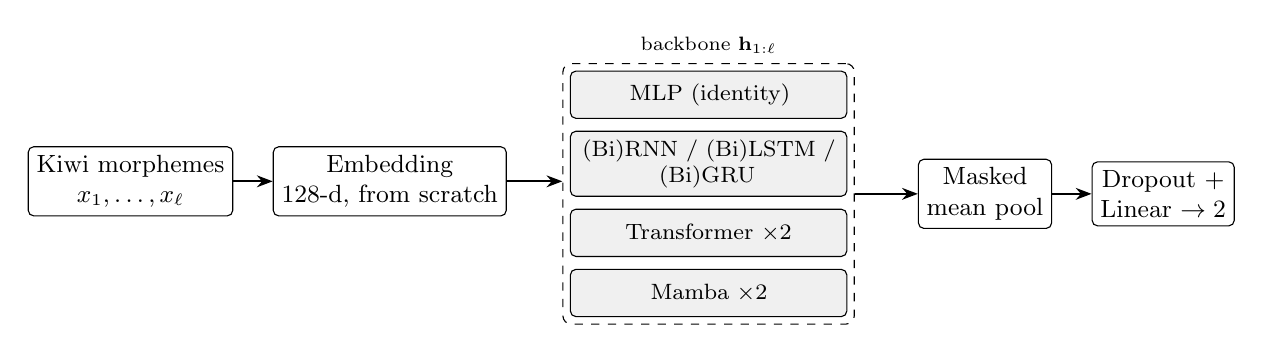
\begin{tikzpicture}[
      node distance=4mm and 5mm,
      box/.style={draw, rounded corners=2pt, minimum height=7mm, align=center, font=\small, inner sep=3pt},
      bb/.style={box, fill=black!6, text width=33mm, minimum height=6mm, font=\footnotesize},
      arr/.style={-{Stealth[length=2mm]}, thick}]
    \node[box] (in) {Kiwi morphemes\\$x_1,\dots,x_\ell$};
    \node[box, right=of in] (emb) {Embedding\\$128$-d, from scratch};
    \node[bb, right=8mm of emb, yshift=11mm] (mlp) {MLP (identity)};
    \node[bb, below=1.5mm of mlp] (rnn) {(Bi)RNN / (Bi)LSTM /\\ (Bi)GRU};
    \node[bb, below=1.5mm of rnn] (trf) {Transformer $\times2$};
    \node[bb, below=1.5mm of trf] (mam) {Mamba $\times2$};
    \node[draw, dashed, rounded corners=3pt, fit=(mlp)(rnn)(trf)(mam), inner sep=2.5pt,
          label={[font=\scriptsize]above:backbone $\mathbf{h}_{1:\ell}$}] (back) {};
    \node[box, right=8mm of back] (pool) {Masked\\mean pool};
    \node[box, right=of pool] (head) {Dropout +\\Linear $\to2$};
    \draw[arr] (in) -- (emb);
    \draw[arr] (emb.east) -- (back.west |- emb.east);
    \draw[arr] (back.east |- pool.west) -- (pool);
    \draw[arr] (pool) -- (head);
  \end{tikzpicture}
  \caption{Shared template of the nine neural classifiers. Only the backbone differs; the
  input, the 128-d embedding, masked mean pooling over valid tokens and the linear head are
  identical. For the MLP the backbone is the identity and the two-layer MLP is applied after
  pooling (deep averaging network).}
  \label{fig:arch}
\end{figure}

\paragraph{MLP (deep averaging network).}
Following DAN~\cite{iyyer2015deep}, the embeddings are pooled first and the pooled vector
passes through two hidden layers of width $w$:
$\mathbf{z}_0=\bar{\mathbf{e}}$, $\mathbf{z}_k=\operatorname{Dropout}(\operatorname{ReLU}(\mathbf{W}_k\mathbf{z}_{k-1}+\mathbf{b}_k))$
for $k=1,2$, followed by the linear head. It ignores word order completely and is the
neural counterpart of a bag-of-words model.

\paragraph{Recurrent networks (RNN, LSTM, GRU and their bidirectional versions).}
Each recurrent model has one layer. The \emph{unidirectional} RNN, LSTM and GRU read the
sequence left-to-right only, $\mathbf{h}_t=\overrightarrow{\mathbf{h}}_t\in\mathbb{R}^{w}$, so
the state at position $t$ has seen only the prefix $x_{1:t}$. The \emph{bidirectional}
BiRNN, BiLSTM and BiGRU add a second, independent layer that reads right-to-left~\cite{schuster1997bidirectional};
$w$ is then the hidden size per direction and
$\mathbf{h}_t=[\overrightarrow{\mathbf{h}}_t;\overleftarrow{\mathbf{h}}_t]\in\mathbb{R}^{2w}$, so
every position sees the whole review. Comparing each pair isolates the value of
right-to-left context at equal parameter count. Sequences are packed, so padding never
enters the recurrence. Within each direction setting the three variants differ only in
the cell (written below for the forward direction). The \textbf{RNN}/\textbf{BiRNN} use the plain Elman cell~\cite{elman1990finding},
$\overrightarrow{\mathbf{h}}_t=\tanh(\mathbf{W}\mathbf{e}_t+\mathbf{U}\overrightarrow{\mathbf{h}}_{t-1}+\mathbf{b})$,
which has no gates and is the baseline for what gating adds.
The \textbf{LSTM}/\textbf{BiLSTM}~\cite{hochreiter1997long} add input, forget and output gates and a
separate memory cell,
$\mathbf{c}_t=\mathbf{f}_t\odot\mathbf{c}_{t-1}+\mathbf{i}_t\odot\tanh(\mathbf{W}_c\mathbf{e}_t+\mathbf{U}_c\mathbf{h}_{t-1}+\mathbf{b}_c)$,
$\mathbf{h}_t=\mathbf{o}_t\odot\tanh(\mathbf{c}_t)$, with each gate
$\sigma(\mathbf{W}_g\mathbf{e}_t+\mathbf{U}_g\mathbf{h}_{t-1}+\mathbf{b}_g)$.
The \textbf{GRU}/\textbf{BiGRU}~\cite{cho2014learning} merge memory and state and use an update
gate $\mathbf{u}_t$ and a reset gate $\mathbf{r}_t$:
$\tilde{\mathbf{h}}_t=\tanh(\mathbf{W}\mathbf{e}_t+\mathbf{U}(\mathbf{r}_t\odot\mathbf{h}_{t-1})+\mathbf{b})$,
$\mathbf{h}_t=(1-\mathbf{u}_t)\odot\mathbf{h}_{t-1}+\mathbf{u}_t\odot\tilde{\mathbf{h}}_t$.
Per direction, an RNN, GRU and LSTM layer has one, three and four weight blocks of
size $w(128+w+2)$ respectively, so at equal budget the plain RNN is the widest, and a
unidirectional model is wider than its bidirectional twin, which splits the budget over
two directions (\cref{tab:arch}).

\paragraph{Transformer encoder.}
The embedding is projected to $d=w$ dimensions and a learned positional embedding
$\mathbf{p}_t$ ($L$ positions) is added: $\mathbf{u}_t=\mathbf{W}_p\mathbf{e}_t+\mathbf{p}_t$.
Two pre-norm encoder layers~\cite{vaswani2017attention} follow, each
$\mathbf{a}=\mathbf{u}+\operatorname{MHSA}(\operatorname{LN}(\mathbf{u}))$,
$\mathbf{u}'=\mathbf{a}+\mathbf{W}_2\operatorname{GELU}(\mathbf{W}_1\operatorname{LN}(\mathbf{a}))$,
with four attention heads, a feed-forward width of $2d$, dropout $p$ inside both
sub-layers, and a key-padding mask so that attention ignores padding. A final
LayerNorm~\cite{ba2016layer} precedes pooling. Positional embeddings are counted as
embedding parameters.

\paragraph{Mamba.}
The embedding is projected to $d=w$ and passed through two pre-norm residual blocks
$\mathbf{x}\leftarrow\mathbf{x}+\operatorname{Mixer}(\operatorname{RMSNorm}(\mathbf{x}))$~\cite{zhang2019root}.
The mixer is the selective state-space layer of \citet{gu2023mamba} with expansion 2
($d_\text{in}=2d$), a causal depthwise convolution of width 4 and state size $N=16$:
$[\tilde{\mathbf{x}},\mathbf{z}]=\mathbf{W}_\text{in}\mathbf{x}$,
$\tilde{\mathbf{x}}\leftarrow\operatorname{SiLU}(\operatorname{conv}(\tilde{\mathbf{x}}))$, and for every
channel
\begin{equation}
  \mathbf{s}_t=\exp(\Delta_t\mathbf{A})\odot\mathbf{s}_{t-1}+\Delta_t\mathbf{B}_t\tilde{x}_t,\qquad
  y_t=\mathbf{C}_t^{\top}\mathbf{s}_t+D\,\tilde{x}_t ,
\end{equation}
where the step size $\Delta_t=\operatorname{softplus}(\cdot)$ (rank $\lceil d/16\rceil$) and
$\mathbf{B}_t,\mathbf{C}_t\in\mathbb{R}^{N}$ are computed from $\tilde{\mathbf{x}}_t$: this
input dependence (``selection'') lets the model decide per token what to keep in its
state. The output is $\mathbf{W}_\text{out}(\mathbf{y}\odot\operatorname{SiLU}(\mathbf{z}))$.
The scan is causal, so right padding cannot affect valid positions; a final RMSNorm
precedes pooling. Mamba has two interchangeable implementations with identical
parameters: the fused CUDA kernels of \texttt{mamba-ssm} and a pure-PyTorch reference
selective scan (\texttt{torch\_ref}); all reported Mamba results use \mambaBackend{}, and CPU
latency always uses \texttt{torch\_ref}.

\paragraph{Parameter matching.}
Each architecture has three width levels S/M/L. For every architecture and level we
search the width $w$ whose non-embedding parameter count is closest to 50k, 200k and
500k respectively; all resulting models lie within $\pm3\%$ of the target
(\cref{tab:arch}). The width level is a tuned hyperparameter (\cref{sec:methods}), so
each dataset may select a different level.

\begin{table}[t]
  \centering
  \caption{Neural architectures. ``Width'' is the size that is varied to meet the
  parameter budget; S/M/L give the width and, in parentheses, the resulting number of
  non-embedding parameters (target in the header). All models additionally have a
  $|V|\times128$ embedding table ($\approx$2.56M parameters at $|V|\approx20$k) and a
  linear output layer.}
  \label{tab:arch}
  % AUTO-GENERATED by ksent.analysis.make_tables (do not edit by hand).
\begin{adjustbox}{max width=\linewidth}
\begin{tabular}{l>{\raggedright\arraybackslash}p{5.2cm}>{\raggedright\arraybackslash}p{2.8cm}lrrr}
\toprule
Method & Backbone & Fixed structure & Width = & S (50.0k) & M (200.0k) & L (500.0k) \\
\midrule
Emb + MLP & masked mean $\to$ 2$\times$[Linear, ReLU, dropout] & 2 hidden layers & hidden units per layer & 167 (49.9k) & 386 (199.9k) & 644 (499.7k) \\
Emb + RNN & 1-layer Elman RNN ($\tanh$), masked mean & 1 layer, 1 dir. & hidden units & 167 (49.9k) & 386 (199.9k) & 644 (499.7k) \\
Emb + LSTM & 1-layer LSTM, masked mean & 1 layer, 1 dir. & hidden units & 64 (49.8k) & 168 (200.6k) & 294 (499.2k) \\
Emb + GRU & 1-layer GRU, masked mean & 1 layer, 1 dir. & hidden units & 79 (49.7k) & 201 (200.0k) & 348 (499.7k) \\
Emb + BiRNN & 1-layer bidirectional Elman RNN ($\tanh$), masked mean & 1 layer, 2 dir. & hidden units per direction & 105 (49.8k) & 257 (199.9k) & 438 (499.3k) \\
Emb + BiLSTM & 1-layer bidirectional LSTM, masked mean & 1 layer, 2 dir. & hidden units per direction & 37 (49.6k) & 106 (200.6k) & 193 (499.5k) \\
Emb + BiGRU & 1-layer bidirectional GRU, masked mean & 1 layer, 2 dir. & hidden units per direction & 47 (50.1k) & 129 (201.0k) & 231 (501.3k) \\
Transformer & Linear 128$\to d$ + learned positions, pre-norm encoder, LayerNorm, masked mean & 2 layers, 4 heads, FFN $2d$, GELU & $d_\text{model}$ & 52 (51.3k) & 108 (203.4k) & 172 (500.0k) \\
Mamba & Linear 128$\to d$, pre-norm residual Mamba blocks, RMSNorm, masked mean & 2 blocks, $d_\text{state}$=16, conv 4, expand 2 & $d_\text{model}$ & 50 (49.3k) & 112 (196.4k) & 186 (498.9k) \\
\bottomrule
\end{tabular}
\end{adjustbox}

\end{table}

\paragraph{Fixed neural training rules.}
AdamW~\cite{loshchilov2019decoupled} (weight decay 0.01), batch size 64, at most 30
epochs, early stopping with patience 5 on validation macro-F1 with the best
checkpoint restored, gradient clipping at 1.0, cross-entropy loss and fp32
precision---identical for every size.

\paragraph{Tuning.}
For each dataset and method we evaluate exactly ten predefined configurations
(\cref{tab:a2defs}) at $n=2{,}000$ with tuning seed 0 and select the one with the
highest validation macro-F1 (ties: lower fit time). The search covers
regularisation for linear models, tree structure and sampling for RF, depth,
learning rate and sampling for XGBoost (whose early-stopped number of rounds is
frozen), and learning rate, dropout and width for neural models. The selected
configuration is frozen for all sizes and seeds; the validation macro-F1 of every tuning
configuration is listed in \cref{tab:a2}.

\begin{sidewaystable}
  \centering
  \caption{Method configurations. ``Selected'' is the frozen configuration per
  dataset (RF: trees, depth, features, minimum leaf size, class weight; XGB: depth,
  learning rate, subsampling, rounds; neural: width level, learning rate, dropout).
  ``Size'' is the non-embedding parameter count (neural), the number of non-zero
  coefficients (LR/SVM) or total tree nodes (RF/XGB) at $n=8{,}000$.
  ``Tune'' is the summed fit time of the ten tuning runs.}
  \label{tab:methods}
  % AUTO-GENERATED by ksent.analysis.make_tables (do not edit by hand).
\begin{adjustbox}{max width=\linewidth}
\begin{tabular}{lllllrrlrrlrr}
\toprule
Method & Family & Representation & Search space & \multicolumn{3}{c}{NSMC} & \multicolumn{3}{c}{Shopping} & \multicolumn{3}{c}{Steam} \\
\cmidrule(lr){5-7}\cmidrule(lr){8-10}\cmidrule(lr){11-13}
 & & & & Selected & Size & Tune (s) & Selected & Size & Tune (s) & Selected & Size & Tune (s) \\
\midrule
TF-IDF + LR & TF-IDF & TF-IDF 1--2-gram & $C\in\{10^{-2},\dots,300\}$ & -- & -- & -- & -- & -- & -- & -- & -- & -- \\
TF-IDF + SVM & TF-IDF & TF-IDF 1--2-gram & $C\in\{10^{-2},\dots,300\}$ & -- & -- & -- & -- & -- & -- & -- & -- & -- \\
TF-IDF + RF & TF-IDF & TF-IDF 1--2-gram & trees, depth, feat., leaf, weight (10/32) & -- & -- & -- & -- & -- & -- & -- & -- & -- \\
TF-IDF + XGBoost & TF-IDF & TF-IDF 1--2-gram & depth, $\eta$, sampling (10/18); rounds by ES & -- & -- & -- & -- & -- & -- & -- & -- & -- \\
\midrule
Emb + MLP & Neural & Emb.\ mean pool & lr, dropout, width S/M/L (10/27) & -- & -- & -- & -- & -- & -- & -- & -- & -- \\
Emb + LSTM & Neural & Emb.\ + BiLSTM & lr, dropout, width S/M/L (10/27) & -- & -- & -- & -- & -- & -- & -- & -- & -- \\
Emb + GRU & Neural & Emb.\ + BiGRU & lr, dropout, width S/M/L (10/27) & -- & -- & -- & -- & -- & -- & -- & -- & -- \\
Transformer & Neural & Emb.\ + 2-layer encoder & lr, dropout, width S/M/L (10/27) & -- & -- & -- & -- & -- & -- & -- & -- & -- \\
Mamba & Neural & Emb.\ + 2 Mamba blocks & lr, dropout, width S/M/L (10/27) & -- & -- & -- & -- & -- & -- & -- & -- & -- \\
\bottomrule
\end{tabular}
\end{adjustbox}

\end{sidewaystable}

\section{Experimental Setup}
\label{sec:setup}

\begin{figure}[t]
  \centering
  % Fig. 1 - experimental pipeline (TikZ). Shared by the report and the slides.
\begin{adjustbox}{max width=\linewidth, max totalheight=0.5\textheight}
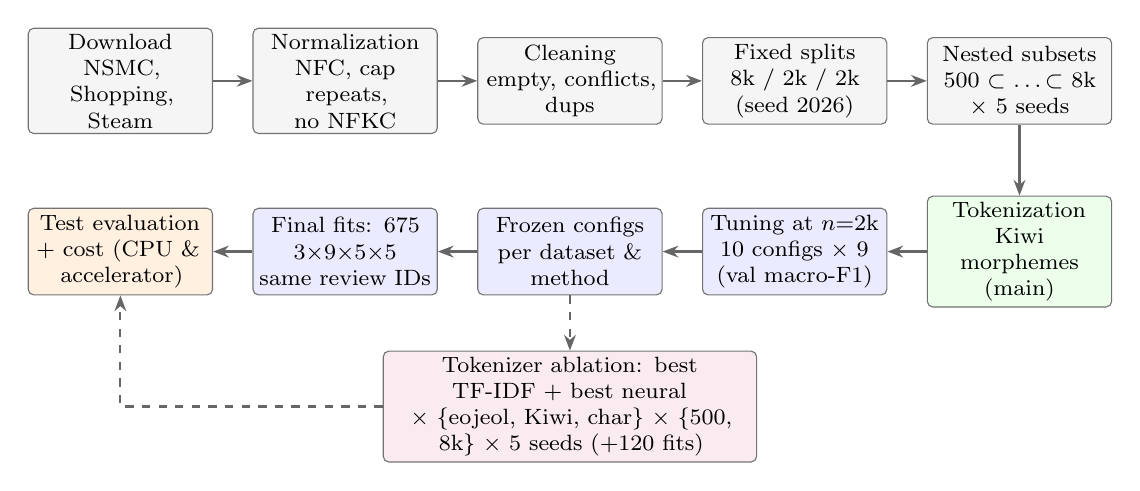
\begin{tikzpicture}[
  node distance=5mm and 5mm,
  box/.style={draw=black!55, rounded corners=2pt, fill=#1, align=center, font=\footnotesize,
              minimum height=11mm, text width=22mm, inner sep=2pt},
  box/.default=black!4,
  arr/.style={-{Stealth[length=2mm]}, thick, black!60},
  lab/.style={font=\scriptsize\itshape, text=black!60}]
  % row 1: data
  \node[box] (dl) {Download\\NSMC, Shopping,\\Steam};
  \node[box, right=of dl] (nm) {Normalization\\NFC, cap repeats,\\no NFKC};
  \node[box, right=of nm] (cl) {Cleaning\\empty, conflicts,\\dups};
  \node[box, right=of cl] (sp) {Fixed splits\\8k / 2k / 2k\\(seed 2026)};
  \node[box, right=of sp] (sub) {Nested subsets\\500 $\subset$ \dots $\subset$ 8k\\$\times$ 5 seeds};
  % row 2: modelling
  \node[box=green!8, below=9mm of sub] (tok) {Tokenization\\Kiwi\\morphemes (main)};
  \node[box=blue!8, left=of tok] (tune) {Tuning at $n$=2k\\10 configs $\times$ 9\\(val macro-F1)};
  \node[box=blue!8, left=of tune] (frz) {Frozen configs\\per dataset \&\\method};
  \node[box=blue!8, left=of frz] (fit) {Final fits: 675\\3$\times$9$\times$5$\times$5\\same review IDs};
  \node[box=orange!12, left=of fit] (ev) {Test evaluation\\+ cost (CPU \&\\accelerator)};
  % row 3: ablation branch
  \node[box=purple!8, below=7mm of frz, text width=46mm] (abl) {Tokenizer ablation: best TF-IDF + best neural\\
    $\times$ \{eojeol, Kiwi, char\} $\times$ \{500, 8k\} $\times$ 5 seeds (+120 fits)};
  \draw[arr] (dl) -- (nm);
  \draw[arr] (nm) -- (cl);
  \draw[arr] (cl) -- (sp);
  \draw[arr] (sp) -- (sub);
  \draw[arr] (sub) -- (tok);
  \draw[arr] (tok) -- (tune);
  \draw[arr] (tune) -- (frz);
  \draw[arr] (frz) -- (fit);
  \draw[arr] (fit) -- (ev);
  \draw[arr, dashed] (frz) -- (abl);
  \draw[arr, dashed] (abl.west) -| (ev.south);
\end{tikzpicture}
\end{adjustbox}

  \caption{Experimental pipeline. Validation data drive tuning, early stopping, the choice
  of the best method per family and of the ablation methods; test data are used once, for
  the final evaluation of frozen pipelines. The dashed branch is the tokenizer ablation.}
  \label{fig:pipeline}
\end{figure}

\paragraph{Protocol.}
\Cref{fig:pipeline} summarises the protocol. Every final condition
(3 datasets $\times$ 13 methods $\times$ 10--14 sizes per dataset) is repeated with \nSeeds{} seeds
(\seedList), giving \nFinalFits{} final fits plus \nTuningFits{} tuning fits.
The seed controls the nested training subset and all model randomness, so the
TF-IDF and neural runs with the same seed see exactly the same reviews.

\paragraph{Metrics.}
Macro-F1 is the primary metric; accuracy, macro-precision and macro-recall are
secondary (\cref{tab:a1acc,tab:a1p,tab:a1r}). We report mean\,$\pm$\,sample standard deviation over seeds; the seeds
measure variability but do not constitute a significance test. Confusion matrices at
$n=8{,}000$ are summed over the \nSeeds{} runs and row-normalised. The marginal value of
labels is the per-seed macro-F1 gain between adjacent sizes.

\paragraph{Crossover threshold.}
At every size we select the best TF-IDF and the best neural method by mean
\emph{validation} macro-F1, compute the test macro-F1 gap (neural minus TF-IDF)
per seed---paired, because both saw the same subset---and average it. The
threshold is the smallest size whose mean gap is at least \crossoverMargin{} point;
otherwise we report ``no observed crossover up to the full training set''. As a sensitivity check we
repeat the procedure with winners selected by test macro-F1 (\cref{tab:a4}). At the
threshold (or at the cost-pass size 8{,}000 if there is none) we check whether the neural winner is
Pareto-efficient against the TF-IDF winner on test macro-F1, CPU end-to-end latency,
fit time and peak RAM.

\paragraph{Cost measurement.}
All runs use one machine (\cpuModel{}; accelerator: \gpuModel; \hardwareNote). Every run
is a separate process with a fixed thread count: \nThreads{} CPU threads for TF-IDF fits
and all CPU inference, and \neuralThreads{} for neural training. We run in two modes. In
\emph{quality} runs, which supply all predictive metrics, jobs run concurrently: up to
\kGpu{} neural jobs share the GPU, and \cpuJobs{} TF-IDF jobs run alongside them. Concurrency
changes neither a job's thread count nor its device. In \emph{cost} runs, which supply
every reported time and memory figure, jobs run one at a time on an otherwise idle machine.
These cover all methods at $n=8{,}000$, the crossover sizes and all tuning fits. We check
that the two modes produce the same test predictions (\cref{sec:results}). Neural
models train on \trainDevice{} in \precisionUsed{}; TF-IDF models always run on the CPU. We record end-to-end fit
time (tokenisation + vectoriser/vocabulary + training) and classifier-only fit time;
batch-size-1 inference latency on 200 fixed test reviews after 20 warm-up calls
(median), both classifier-only (pre-vectorised input) and end-to-end (raw string to
label), on the CPU for every method (the primary, comparable measurement) and
additionally on the accelerator (\accelDevice) for neural methods, with device
synchronisation around every call; peak host RAM of the process; peak accelerator
memory; serialised artefact size; and model size
(parameters, non-zero coefficients or tree nodes). Hardware and software versions
are listed in \cref{tab:a6}. As a check on the two-mode design, every cost run was compared
with its quality run: \detIdentical{} of \detRuns{} runs produced identical test
predictions (maximum disagreement \detMaxDisagree), so concurrency did not affect any
predictive result.

\paragraph{Compute used.}
All experiments ran on a single machine with one \gpuModel{} and a \cpuModel{},
in \precisionUsed. Busy wall-clock time per stage, from the first job start to the last job
end, was: pilot \wallPilot{}\,h, tuning \wallTuning{}\,h (exclusive), main sweep
\wallSweep{}\,h (parallel, mean GPU utilisation \gpuUtilSweep), tokenizer ablation
\wallAblation{}\,h (parallel, \gpuUtilAblation) and cost pass \wallCostPass{}\,h
(exclusive). The total is \wallTotal{}\,h, i.e.\ \wallTotal{} GPU-hours on one GPU; the
neural jobs alone add up to \gpuJobHours{}\,h of job time, because up to \kGpu{} of them
shared the GPU. The exclusive stages leave the GPU mostly idle (\gpuUtilTuning{} in tuning,
\gpuUtilCostPass{} in the cost pass), as they must for undisturbed timings.

\paragraph{Deviations from the proposal.}
(i) \nSeeds{} seeds instead of 3, i.e.\ \nFinalFits{} instead of 405 final fits; confusion
matrices are summed over \nSeeds{} runs. Tuning is unchanged (\nTuningFits{} fits).
(ii) A tokenizer ablation (\cref{sec:ablation}, \nAblationFits{} additional fits) that was not
planned. (iii) Preprocessing is specified in more detail than in the proposal (fixed
normalization rules, Kiwi morphemes with POS tags, \cref{sec:preprocessing}).
(iv) All results are reported as mean\,$\pm$\,sample standard deviation over \nSeeds{} seeds.
(v) Cost figures (fit time, latency, memory) are measured in separate exclusive cost runs.
These cover all methods at $n=8{,}000$ and the crossover sizes; they are not measured at every
training size.
(vi) Mamba uses the pure-PyTorch selective scan (\mambaBackend{}), because no
\texttt{mamba-ssm} build exists for the PyTorch version we used. Its fit time and GPU latency are
therefore probably higher than the fused kernels would give.
(vii) Because no crossover was observed, no additional cost runs at a crossover size were
needed; all cost figures refer to $n=8{,}000$.
(viii) The size grid is extended beyond the proposal's maximum of 8{,}000 reviews with
16{,}000, 32{,}000, 64{,}000, steps of 20{,}000 up to 160{,}000 and the full training set
(\cref{sec:data}), so the learning
curves reach the point where all available labels are used. Cost runs stay at
$n=8{,}000$ (plus any crossover size).
(ix) Three recurrent baselines are added: a plain bidirectional Elman RNN (BiRNN), which
separates the effect of recurrence from that of gating in the BiLSTM and BiGRU, and
unidirectional RNN, LSTM and GRU, which isolate the effect of bidirectionality
(\cref{sec:arch}); the proposal's LSTM and GRU are the bidirectional ones.

\section{Results}
\label{sec:results}

\subsection{Learning curves}

\begin{figure}[t]
  \centering
  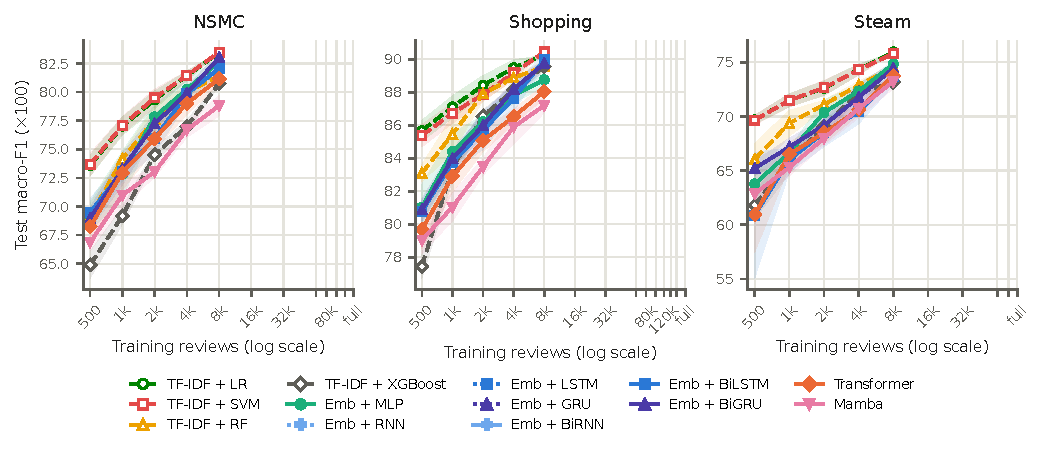
\includegraphics[width=\linewidth]{figures/fig2_learning_curves.pdf}
  \caption{Learning curves: test macro-F1 versus training size (log scale) for all
  thirteen methods; shaded bands are $\pm1$ standard deviation over \nSeeds{} seeds
  (sample std, ddof\,=\,1). Dashed lines with hollow markers are TF-IDF methods;
  solid lines with filled markers are neural methods. The dotted vertical line marks
  the crossover threshold when one exists.}
  \label{fig:curves}
\end{figure}

\begin{table}[t]
  \centering
  \caption{Test macro-F1 ($\times100$) across training sizes. \pmnote{} Bold: best
  mean in the column within each dataset. $^{\dagger}$/$^{\ddagger}$: best TF-IDF /
  best neural method at that size, selected by validation macro-F1 (the pair used for
  the crossover).}
  \label{tab:f1}
  % AUTO-GENERATED by ksent.analysis.make_tables (do not edit by hand).
\begin{adjustbox}{max width=\linewidth}
\begin{tabular}{lrrrrrrrrrrrrrr}
\toprule
Method & $n$=500 & $n$=1{,}000 & $n$=2{,}000 & $n$=4{,}000 & $n$=8{,}000 & $n$=16{,}000 & $n$=32{,}000 & $n$=64{,}000 & $n$=80{,}000 & $n$=100{,}000 & $n$=120{,}000 & $n$=140{,}000 & $n$=160{,}000 & full \\
\midrule
\multicolumn{15}{l}{\textit{NSMC} (full = 143{,}640)} \\
TF-IDF + LR & 73.59{\scriptsize$\pm$0.89} & 77.03{\scriptsize$\pm$0.77} & 79.32{\scriptsize$\pm$0.76} & 81.43{\scriptsize$\pm$0.40}$^{\dagger}$ & 83.45{\scriptsize$\pm$0.00} & -- & -- & -- & -- & -- & -- &  &  & -- \\
TF-IDF + SVM & \textbf{73.67}{\scriptsize$\pm$0.95}$^{\dagger}$ & \textbf{77.10}{\scriptsize$\pm$0.75}$^{\dagger}$ & \textbf{79.49}{\scriptsize$\pm$0.75}$^{\dagger}$ & \textbf{81.45}{\scriptsize$\pm$0.39} & \textbf{83.50}{\scriptsize$\pm$0.00}$^{\dagger}$ & -- & -- & -- & -- & -- & -- &  &  & -- \\
TF-IDF + RF & 69.13{\scriptsize$\pm$1.11} & 74.15{\scriptsize$\pm$0.53} & 77.63{\scriptsize$\pm$1.06} & 79.98{\scriptsize$\pm$0.66} & 81.43{\scriptsize$\pm$0.23} & -- & -- & -- & -- & -- & -- &  &  & -- \\
TF-IDF + XGBoost & 64.90{\scriptsize$\pm$1.15} & 69.19{\scriptsize$\pm$0.73} & 74.54{\scriptsize$\pm$0.50} & 77.01{\scriptsize$\pm$0.55} & 80.76{\scriptsize$\pm$0.14} & -- & -- & -- & -- & -- & -- &  &  & -- \\
\cmidrule(lr){1-15}
Emb + MLP & 69.16{\scriptsize$\pm$1.29} & 72.84{\scriptsize$\pm$1.99} & 77.84{\scriptsize$\pm$1.04}$^{\ddagger}$ & 80.24{\scriptsize$\pm$0.78}$^{\ddagger}$ & 82.65{\scriptsize$\pm$0.40} & -- & -- & -- & -- & -- & -- &  &  & -- \\
Emb + RNN & -- & -- & -- & -- & -- & -- & -- & -- & -- & -- & -- &  &  & -- \\
Emb + LSTM & -- & -- & -- & -- & -- & -- & -- & -- & -- & -- & -- &  &  & -- \\
Emb + GRU & -- & -- & -- & -- & -- & -- & -- & -- & -- & -- & -- &  &  & -- \\
Emb + BiRNN & -- & -- & -- & -- & -- & -- & -- & -- & -- & -- & -- &  &  & -- \\
Emb + BiLSTM & 69.50{\scriptsize$\pm$1.22} & 73.06{\scriptsize$\pm$0.83} & 75.96{\scriptsize$\pm$1.32} & 79.84{\scriptsize$\pm$0.70} & 82.08{\scriptsize$\pm$0.64} & -- & -- & -- & -- & -- & -- &  &  & -- \\
Emb + BiGRU & 68.96{\scriptsize$\pm$0.96}$^{\ddagger}$ & 73.26{\scriptsize$\pm$1.35}$^{\ddagger}$ & 77.23{\scriptsize$\pm$0.86} & 79.89{\scriptsize$\pm$0.51} & 83.02{\scriptsize$\pm$0.49}$^{\ddagger}$ & -- & -- & -- & -- & -- & -- &  &  & -- \\
Transformer & 68.25{\scriptsize$\pm$1.12} & 72.96{\scriptsize$\pm$1.48} & 75.92{\scriptsize$\pm$0.90} & 79.02{\scriptsize$\pm$0.96} & 81.16{\scriptsize$\pm$0.44} & -- & -- & -- & -- & -- & -- &  &  & -- \\
Mamba & 66.88{\scriptsize$\pm$0.73} & 71.00{\scriptsize$\pm$1.02} & 73.03{\scriptsize$\pm$0.44} & 76.71{\scriptsize$\pm$0.66} & 78.81{\scriptsize$\pm$0.87} & -- & -- & -- & -- & -- & -- &  &  & -- \\
\midrule
\multicolumn{15}{l}{\textit{Shopping} (full = 195{,}881)} \\
TF-IDF + LR & \textbf{85.67}{\scriptsize$\pm$0.62}$^{\dagger}$ & \textbf{87.11}{\scriptsize$\pm$0.66}$^{\dagger}$ & \textbf{88.42}{\scriptsize$\pm$0.59}$^{\dagger}$ & \textbf{89.49}{\scriptsize$\pm$0.47}$^{\dagger}$ & 90.25{\scriptsize$\pm$0.00} & -- & -- & -- & -- & -- & -- & -- & -- & -- \\
TF-IDF + SVM & 85.37{\scriptsize$\pm$0.67} & 86.73{\scriptsize$\pm$0.61} & 87.87{\scriptsize$\pm$0.41} & 89.17{\scriptsize$\pm$0.37} & \textbf{90.45}{\scriptsize$\pm$0.00}$^{\dagger}$ & -- & -- & -- & -- & -- & -- & -- & -- & -- \\
TF-IDF + RF & 83.09{\scriptsize$\pm$0.51} & 85.46{\scriptsize$\pm$1.10} & 87.90{\scriptsize$\pm$0.39} & 88.87{\scriptsize$\pm$0.13} & 89.55{\scriptsize$\pm$0.33} & -- & -- & -- & -- & -- & -- & -- & -- & -- \\
TF-IDF + XGBoost & 77.44{\scriptsize$\pm$0.71} & 83.42{\scriptsize$\pm$0.75} & 86.56{\scriptsize$\pm$0.36} & 88.13{\scriptsize$\pm$0.31} & 89.57{\scriptsize$\pm$0.22} & -- & -- & -- & -- & -- & -- & -- & -- & -- \\
\cmidrule(lr){1-15}
Emb + MLP & 81.04{\scriptsize$\pm$1.39}$^{\ddagger}$ & 84.40{\scriptsize$\pm$1.09}$^{\ddagger}$ & 86.21{\scriptsize$\pm$0.39}$^{\ddagger}$ & 87.83{\scriptsize$\pm$0.47} & 88.76{\scriptsize$\pm$0.39} & -- & -- & -- & -- & -- & -- & -- & -- & -- \\
Emb + RNN & -- & -- & -- & -- & -- & -- & -- & -- & -- & -- & -- & -- & -- & -- \\
Emb + LSTM & -- & -- & -- & -- & -- & -- & -- & -- & -- & -- & -- & -- & -- & -- \\
Emb + GRU & -- & -- & -- & -- & -- & -- & -- & -- & -- & -- & -- & -- & -- & -- \\
Emb + BiRNN & -- & -- & -- & -- & -- & -- & -- & -- & -- & -- & -- & -- & -- & -- \\
Emb + BiLSTM & 80.77{\scriptsize$\pm$0.67} & 83.75{\scriptsize$\pm$0.49} & 85.69{\scriptsize$\pm$1.16} & 87.64{\scriptsize$\pm$0.77} & 89.96{\scriptsize$\pm$0.39}$^{\ddagger}$ & -- & -- & -- & -- & -- & -- & -- & -- & -- \\
Emb + BiGRU & 80.87{\scriptsize$\pm$0.66} & 83.99{\scriptsize$\pm$0.56} & 85.98{\scriptsize$\pm$0.63} & 88.19{\scriptsize$\pm$0.51}$^{\ddagger}$ & 89.74{\scriptsize$\pm$0.20} & -- & -- & -- & -- & -- & -- & -- & -- & -- \\
Transformer & 79.69{\scriptsize$\pm$1.17} & 82.90{\scriptsize$\pm$0.95} & 85.08{\scriptsize$\pm$0.67} & 86.52{\scriptsize$\pm$0.44} & 88.04{\scriptsize$\pm$0.41} & -- & -- & -- & -- & -- & -- & -- & -- & -- \\
Mamba & 79.04{\scriptsize$\pm$0.81} & 81.04{\scriptsize$\pm$0.84} & 83.48{\scriptsize$\pm$0.50} & 85.89{\scriptsize$\pm$1.03} & 87.20{\scriptsize$\pm$0.44} & -- & -- & -- & -- & -- & -- & -- & -- & -- \\
\midrule
\multicolumn{15}{l}{\textit{Steam} (full = 95{,}774)} \\
TF-IDF + LR & \textbf{69.68}{\scriptsize$\pm$0.39}$^{\dagger}$ & \textbf{71.49}{\scriptsize$\pm$0.59} & 72.60{\scriptsize$\pm$0.66}$^{\dagger}$ & \textbf{74.33}{\scriptsize$\pm$0.48}$^{\dagger}$ & \textbf{75.95}{\scriptsize$\pm$0.00}$^{\dagger}$ & -- & -- & -- & -- &  &  &  &  & -- \\
TF-IDF + SVM & 69.66{\scriptsize$\pm$0.44} & 71.48{\scriptsize$\pm$0.58}$^{\dagger}$ & \textbf{72.64}{\scriptsize$\pm$0.67} & 74.30{\scriptsize$\pm$0.46} & 75.80{\scriptsize$\pm$0.00} & -- & -- & -- & -- &  &  &  &  & -- \\
TF-IDF + RF & 66.03{\scriptsize$\pm$1.49} & 69.37{\scriptsize$\pm$1.18} & 71.09{\scriptsize$\pm$0.40} & 72.89{\scriptsize$\pm$0.34} & 74.49{\scriptsize$\pm$0.24} & -- & -- & -- & -- &  &  &  &  & -- \\
TF-IDF + XGBoost & 61.78{\scriptsize$\pm$1.19} & 65.98{\scriptsize$\pm$1.27} & 69.04{\scriptsize$\pm$0.73} & 72.20{\scriptsize$\pm$0.53} & 73.15{\scriptsize$\pm$0.18} & -- & -- & -- & -- &  &  &  &  & -- \\
\cmidrule(lr){1-15}
Emb + MLP & 63.77{\scriptsize$\pm$1.31} & 66.64{\scriptsize$\pm$0.44} & 70.36{\scriptsize$\pm$1.16} & 72.34{\scriptsize$\pm$0.61}$^{\ddagger}$ & 74.83{\scriptsize$\pm$0.24}$^{\ddagger}$ & -- & -- & -- & -- &  &  &  &  & -- \\
Emb + RNN & -- & -- & -- & -- & -- & -- & -- & -- & -- &  &  &  &  & -- \\
Emb + LSTM & -- & -- & -- & -- & -- & -- & -- & -- & -- &  &  &  &  & -- \\
Emb + GRU & -- & -- & -- & -- & -- & -- & -- & -- & -- &  &  &  &  & -- \\
Emb + BiRNN & -- & -- & -- & -- & -- & -- & -- & -- & -- &  &  &  &  & -- \\
Emb + BiLSTM & 60.87{\scriptsize$\pm$5.79} & 66.00{\scriptsize$\pm$1.10} & 68.52{\scriptsize$\pm$1.30} & 70.42{\scriptsize$\pm$1.08} & 73.66{\scriptsize$\pm$0.76} & -- & -- & -- & -- &  &  &  &  & -- \\
Emb + BiGRU & 65.20{\scriptsize$\pm$0.67}$^{\ddagger}$ & 67.18{\scriptsize$\pm$0.80}$^{\ddagger}$ & 69.17{\scriptsize$\pm$0.60}$^{\ddagger}$ & 71.76{\scriptsize$\pm$1.24} & 74.43{\scriptsize$\pm$0.52} & -- & -- & -- & -- &  &  &  &  & -- \\
Transformer & 60.95{\scriptsize$\pm$3.49} & 66.51{\scriptsize$\pm$1.08} & 68.48{\scriptsize$\pm$0.98} & 70.63{\scriptsize$\pm$0.46} & 73.75{\scriptsize$\pm$0.40} & -- & -- & -- & -- &  &  &  &  & -- \\
Mamba & 62.87{\scriptsize$\pm$0.76} & 65.29{\scriptsize$\pm$0.77} & 67.98{\scriptsize$\pm$0.64} & 70.73{\scriptsize$\pm$0.83} & 73.22{\scriptsize$\pm$0.63} & -- & -- & -- & -- &  &  &  &  & -- \\
\bottomrule
\end{tabular}
\end{adjustbox}

\end{table}

\Cref{fig:curves} and \cref{tab:f1} show test macro-F1 for every method and size.
At $n=8{,}000$ the best method is \bestMethodNSMC{} on NSMC
(\macroFOneBestNSMC), \bestMethodShopping{} on Shopping (\macroFOneBestShopping)
and \bestMethodSteam{} on Steam (\macroFOneBestSteam).
TF-IDF leads clearly at the smallest size: at $n=500$ the best neural method trails the
best TF-IDF method (both Kiwi-tokenised, selected on validation) by \ablationGapSmallNSMC{}
(NSMC), \ablationGapSmallShopping{} (Shopping) and \ablationGapSmallSteam{} (Steam) points.
Neural curves rise faster, so the gap narrows with data, but the curves of the two family
winners never cross on any dataset: at $n=8{,}000$ the gap is still \gapNSMC,
\gapShopping{} and \gapSteam{} points. One plausible reason for the slow neural start is
vocabulary coverage. With the neural vocabulary built from the training subset
(min.\ frequency 2), \oovSmallNSMC{} (NSMC), \oovSmallShopping{} (Shopping) and
\oovSmallSteam{} (Steam) of test tokens are out of vocabulary at $n=500$, against
\oovLargeNSMC, \oovLargeShopping{} and \oovLargeSteam{} at $n=8{,}000$ (\cref{fig:oov}).
Embeddings trained from scratch on a few thousand reviews have little signal for rare
morphemes, whereas sublinear TF-IDF with a linear model needs no learned representation.
Among the TF-IDF methods, linear models (LR, SVM) dominate RF and XGBoost at every size.
Among the neural methods, the simple embedding models (MLP, GRU, LSTM) are ahead of the
Transformer and Mamba (\cref{sec:discussion}). No method has saturated by $n=8{,}000$
(\cref{sec:marginal}).

\subsection{Crossover thresholds}

\begin{sidewaystable}
  \centering
  \caption{Crossover threshold and cost by dataset. Winners are chosen per size by
  validation macro-F1; the threshold is the smallest size where the mean paired test
  macro-F1 gap (neural $-$ TF-IDF, points) is at least \crossoverMargin. Gap and costs
  are reported at the threshold, or at $n=8{,}000$ when there is no crossover. \pmnote{}
  ``Pareto'': the neural winner is not dominated by the TF-IDF winner on (macro-F1,
  CPU latency, fit time, peak RAM).}
  \label{tab:crossover}
  % AUTO-GENERATED by ksent.analysis.make_tables (do not edit by hand).
\begin{adjustbox}{max width=\linewidth}
\begin{tabular}{lllrrrrrrrrc}
\toprule
Dataset & Best TF-IDF & Best neural & Threshold & Gap (pts) & \multicolumn{2}{c}{Fit e2e (s)} & \multicolumn{2}{c}{CPU e2e latency (ms)} & \multicolumn{2}{c}{Peak RAM (MB)} & Pareto \\
\cmidrule(lr){6-7}\cmidrule(lr){8-9}\cmidrule(lr){10-11}
 & & & & & TF-IDF & Neural & TF-IDF & Neural & TF-IDF & Neural & \\
\midrule
NSMC & TF-IDF + SVM & Emb + BiGRU & none $\le$ full$^{*}$ & -0.48{\scriptsize$\pm$0.49} & 0.898{\scriptsize$\pm$0.077} & 48.8{\scriptsize$\pm$10.1} & 1.04{\scriptsize$\pm$0.06} & 1.21{\scriptsize$\pm$0.01} & 1,445{\scriptsize$\pm$7} & 2,375{\scriptsize$\pm$4} & no \\
Shopping & TF-IDF + SVM & Emb + BiLSTM & none $\le$ full$^{*}$ & -0.49{\scriptsize$\pm$0.39} & 0.997{\scriptsize$\pm$0.089} & 61.1{\scriptsize$\pm$10.6} & 1.04{\scriptsize$\pm$0.07} & 1.50{\scriptsize$\pm$0.02} & 1,453{\scriptsize$\pm$16} & 2,429{\scriptsize$\pm$10} & no \\
Steam & TF-IDF + LR & Emb + MLP & none $\le$ full$^{*}$ & -1.12{\scriptsize$\pm$0.24} & 1.28{\scriptsize$\pm$0.13} & 14.5{\scriptsize$\pm$4.7} & 1.16{\scriptsize$\pm$0.05} & 0.826{\scriptsize$\pm$0.327} & 1,461{\scriptsize$\pm$10} & 2,282{\scriptsize$\pm$10} & yes \\
\bottomrule
\end{tabular}
\end{adjustbox}

\end{sidewaystable}

\Cref{tab:crossover} answers the research question. The crossover threshold is
\crossoverNSMC{} for NSMC (\bestNeuralNSMC{} vs \bestTfidfNSMC, gap \gapNSMC{} points),
\crossoverShopping{} for Shopping (\bestNeuralShopping{} vs \bestTfidfShopping, gap
\gapShopping) and \crossoverSteam{} for Steam (\bestNeuralSteam{} vs \bestTfidfSteam,
gap \gapSteam). Selecting the winners by test instead of validation macro-F1 gives
thresholds of \crossoverTestSelNSMC, \crossoverTestSelShopping{} and
\crossoverTestSelSteam{} (\cref{tab:a4}). The sensitivity check does not change the conclusion. At $n=8{,}000$ validation and test
selection pick the same pair of winners on every dataset. At smaller sizes they sometimes
pick a different pair, but every gap is negative under both rules, so no gap reaches
\crossoverMargin{} point at any size. The research question therefore has the same answer in all three domains:
\emph{no observed crossover up to 8{,}000 reviews}.

\subsection{Quality and cost at 8,000 reviews}

\begin{table}[t]
  \centering
  \caption{Predictive quality at $n=8{,}000$ ($\times100$; from the parallel quality runs).
  \pmnote{} Bold: best per column within a dataset.}
  \label{tab:quality8k}
  % AUTO-GENERATED by ksent.analysis.make_tables (do not edit by hand).
\begin{adjustbox}{max width=\linewidth}
\begin{tabular}{lrrrr}
\toprule
Method & Macro-F1 & Accuracy & Macro-P & Macro-R \\
\midrule
\multicolumn{5}{l}{\textit{NSMC}} \\
TF-IDF + LR & -- & -- & -- & -- \\
TF-IDF + SVM & -- & -- & -- & -- \\
TF-IDF + RF & -- & -- & -- & -- \\
TF-IDF + XGBoost & -- & -- & -- & -- \\
\cmidrule(lr){1-5}
Emb + MLP & -- & -- & -- & -- \\
Emb + LSTM & -- & -- & -- & -- \\
Emb + GRU & -- & -- & -- & -- \\
Transformer & -- & -- & -- & -- \\
Mamba & -- & -- & -- & -- \\
\midrule
\multicolumn{5}{l}{\textit{Shopping}} \\
TF-IDF + LR & -- & -- & -- & -- \\
TF-IDF + SVM & -- & -- & -- & -- \\
TF-IDF + RF & -- & -- & -- & -- \\
TF-IDF + XGBoost & -- & -- & -- & -- \\
\cmidrule(lr){1-5}
Emb + MLP & -- & -- & -- & -- \\
Emb + LSTM & -- & -- & -- & -- \\
Emb + GRU & -- & -- & -- & -- \\
Transformer & -- & -- & -- & -- \\
Mamba & -- & -- & -- & -- \\
\midrule
\multicolumn{5}{l}{\textit{Steam}} \\
TF-IDF + LR & -- & -- & -- & -- \\
TF-IDF + SVM & -- & -- & -- & -- \\
TF-IDF + RF & -- & -- & -- & -- \\
TF-IDF + XGBoost & -- & -- & -- & -- \\
\cmidrule(lr){1-5}
Emb + MLP & -- & -- & -- & -- \\
Emb + LSTM & -- & -- & -- & -- \\
Emb + GRU & -- & -- & -- & -- \\
Transformer & -- & -- & -- & -- \\
Mamba & -- & -- & -- & -- \\
\bottomrule
\end{tabular}
\end{adjustbox}

\end{table}

\begin{sidewaystable}
  \centering
  \caption{Computational cost at $n=8{,}000$. \pmnote{} Fit times in seconds (end-to-end
  includes tokenisation and vectoriser/vocabulary construction); latency is the median
  per-review time at batch size 1 in milliseconds; ``Tune'' is the total fit time of the ten
  tuning runs (single seed); RAM is the peak resident memory of the run's process. Bold:
  lowest cost per column within a dataset. Hardware: \cpuModel{} with \nThreads{} threads
  (CPU columns) and \gpuModel{} (accelerator columns); precision \precisionUsed. Every cost
  comes from exclusive cost runs (one job at a time on an otherwise idle machine), whose
  predictions were identical to the parallel quality runs that supply all predictive
  metrics (\cref{tab:quality8k}).}
  \label{tab:cost}
  % AUTO-GENERATED by ksent.analysis.make_tables (do not edit by hand).
\begin{adjustbox}{max width=\linewidth}
\begin{tabular}{lrrrrrrrrr}
\toprule
Method & Fit e2e (s) & Fit clf.\ (s) & Tune (s) & CPU e2e (ms) & CPU clf.\ (ms) & Accel.\ e2e (ms) & RAM (MB) & Accel.\ mem (MB) & Size (MB) \\
\midrule
\multicolumn{10}{l}{\textit{NSMC}} \\
TF-IDF + LR & -- & -- & -- & -- & -- & n/a & -- & n/a & -- \\
TF-IDF + SVM & -- & -- & -- & -- & -- & n/a & -- & n/a & -- \\
TF-IDF + RF & -- & -- & -- & -- & -- & n/a & -- & n/a & -- \\
TF-IDF + XGBoost & -- & -- & -- & -- & -- & n/a & -- & n/a & -- \\
\cmidrule(lr){1-10}
Emb + MLP & -- & -- & -- & -- & -- & -- & -- & -- & -- \\
Emb + LSTM & -- & -- & -- & -- & -- & -- & -- & -- & -- \\
Emb + GRU & -- & -- & -- & -- & -- & -- & -- & -- & -- \\
Transformer & -- & -- & -- & -- & -- & -- & -- & -- & -- \\
Mamba & -- & -- & -- & -- & -- & -- & -- & -- & -- \\
\midrule
\multicolumn{10}{l}{\textit{Shopping}} \\
TF-IDF + LR & -- & -- & -- & -- & -- & n/a & -- & n/a & -- \\
TF-IDF + SVM & -- & -- & -- & -- & -- & n/a & -- & n/a & -- \\
TF-IDF + RF & -- & -- & -- & -- & -- & n/a & -- & n/a & -- \\
TF-IDF + XGBoost & -- & -- & -- & -- & -- & n/a & -- & n/a & -- \\
\cmidrule(lr){1-10}
Emb + MLP & -- & -- & -- & -- & -- & -- & -- & -- & -- \\
Emb + LSTM & -- & -- & -- & -- & -- & -- & -- & -- & -- \\
Emb + GRU & -- & -- & -- & -- & -- & -- & -- & -- & -- \\
Transformer & -- & -- & -- & -- & -- & -- & -- & -- & -- \\
Mamba & -- & -- & -- & -- & -- & -- & -- & -- & -- \\
\midrule
\multicolumn{10}{l}{\textit{Steam}} \\
TF-IDF + LR & -- & -- & -- & -- & -- & n/a & -- & n/a & -- \\
TF-IDF + SVM & -- & -- & -- & -- & -- & n/a & -- & n/a & -- \\
TF-IDF + RF & -- & -- & -- & -- & -- & n/a & -- & n/a & -- \\
TF-IDF + XGBoost & -- & -- & -- & -- & -- & n/a & -- & n/a & -- \\
\cmidrule(lr){1-10}
Emb + MLP & -- & -- & -- & -- & -- & -- & -- & -- & -- \\
Emb + LSTM & -- & -- & -- & -- & -- & -- & -- & -- & -- \\
Emb + GRU & -- & -- & -- & -- & -- & -- & -- & -- & -- \\
Transformer & -- & -- & -- & -- & -- & -- & -- & -- & -- \\
Mamba & -- & -- & -- & -- & -- & -- & -- & -- & -- \\
\bottomrule
\end{tabular}
\end{adjustbox}

\end{sidewaystable}

\begin{figure}[t]
  \centering
  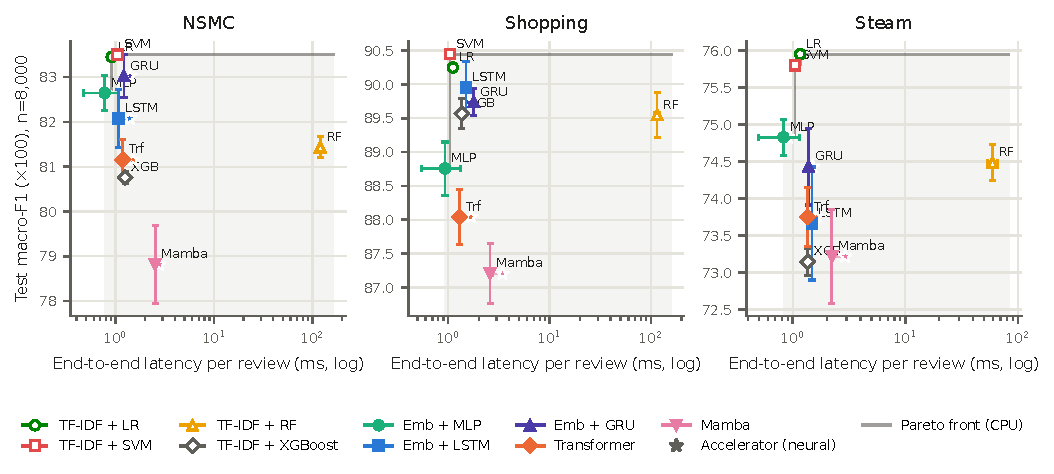
\includegraphics[width=\linewidth]{figures/fig3_quality_vs_cost.pdf}
  \caption{Quality versus inference cost at $n=8{,}000$: test macro-F1 against
  end-to-end CPU latency per review (log scale), error bars $\pm1$ std over \nSeeds{}
  seeds (sample std). Stars connected to neural points show the same model's latency on
  the accelerator (\accelDevice). The grey step line and shaded region mark the CPU Pareto front.}
  \label{fig:cost}
\end{figure}

\Cref{tab:quality8k,tab:cost} and \cref{fig:cost} compare all methods at the largest size.
At the crossover (or at 8{,}000), the neural winner's CPU latency per review is \latencyRatioNSMC{} (NSMC),
\latencyRatioShopping{} (Shopping) and \latencyRatioSteam{} (Steam) that of the TF-IDF
winner, and takes \fitRatioNSMC, \fitRatioShopping{} and
\fitRatioSteam{} longer to fit. It is Pareto-efficient on NSMC: \paretoNSMC;
Shopping: \paretoShopping; Steam: \paretoSteam.
Because there is no crossover, the comparison is made at $n=8{,}000$, where the neural
winner is still \emph{less} accurate. Training is where the two families differ most:
the neural winner needs \fitRatioNSMC, \fitRatioShopping{} and \fitRatioSteam{} the
end-to-end fit time of the TF-IDF winner, and its process peaks at \ramRatioNSMC,
\ramRatioShopping{} and \ramRatioSteam{} the host RAM (the latter mostly reflects the
PyTorch runtime, not the model). Batch-size-1 CPU latency, in contrast, is about one
millisecond for both families (TF-IDF winner \tfidfLatencyNSMC/\tfidfLatencyShopping/\tfidfLatencySteam{} ms,
neural winner \neuralLatencyNSMC/\neuralLatencyShopping/\neuralLatencySteam{} ms on
NSMC/Shopping/Steam). The accelerator does not help at this batch size: the neural winner
takes \neuralAccLatencyNSMC/\neuralAccLatencyShopping/\neuralAccLatencySteam{} ms per
review on the GPU, because kernel launch and host--device transfer dominate a single short
review. The Steam neural winner (Emb\,+\,MLP) is formally Pareto-efficient only because
its mean-pooling network is faster per review than TF-IDF\,+\,LR on the CPU. It is still
\gapSteam{} points less accurate, takes longer to fit and uses more memory, so this is not a
practical argument for switching. Random Forest is the one method whose inference cost
stands out: hundreds of deep trees make it by far the slowest per review and, on Shopping,
by far the largest artefact (\cref{tab:cost}).

\subsection{Class-specific errors}

\begin{figure}[t]
  \centering
  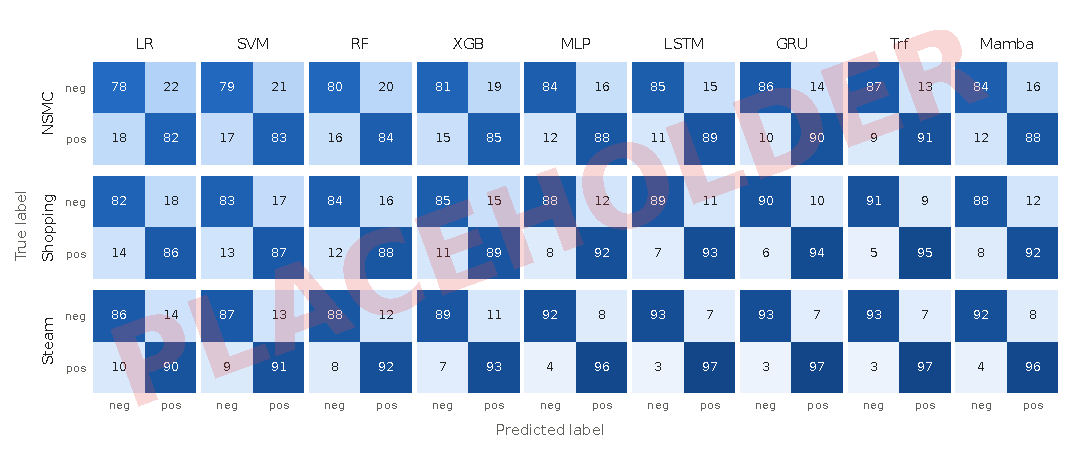
\includegraphics[width=\linewidth]{figures/fig4_confusion.pdf}
  \caption{Confusion matrices at $n=8{,}000$ (rows: true label, columns: predicted),
  counts summed over the \nSeeds{} runs and then row-normalised; cells show
  percentages.}
  \label{fig:confusion}
\end{figure}

\Cref{fig:confusion} shows where the errors fall. On NSMC both winners err at similar
rates on the two classes (TF-IDF: \fprTfidfNSMC{} of negatives predicted positive,
\fnrTfidfNSMC{} of positives predicted negative; neural: \fprNeuralNSMC{} and
\fnrNeuralNSMC). On Shopping the families err in opposite directions: TF-IDF misses more
positives (\fnrTfidfShopping{} vs \fprTfidfShopping), whereas the neural winner
mislabels more negatives (\fprNeuralShopping{} vs \fnrNeuralShopping). This
complementarity suggests that an ensemble could help, which we did not test. Steam is the
hardest domain for both classes and both families: about a quarter of the reviews in
each class are misclassified (TF-IDF \fprTfidfSteam/\fnrTfidfSteam, neural
\fprNeuralSteam/\fnrNeuralSteam), with positives slightly harder. This is consistent with
recommendation flags being a noisy proxy for the sentiment of the text (\cref{sec:limitations}).

\subsection{Marginal value of labels}
\label{sec:marginal}
Doubling the data from 500 to 1{,}000 reviews improves the best 8{,}000-review method by
\gainFirstNSMC, \gainFirstShopping{} and \gainFirstSteam{} points on NSMC, Shopping and
Steam, whereas the last doubling (4{,}000 $\to$ 8{,}000) adds \gainLastNSMC,
\gainLastShopping{} and \gainLastSteam{} points (all gains in \cref{tab:a3}).
None of the curves has flattened. The best TF-IDF method still gains \gainLastNSMC,
\gainLastShopping{} and \gainLastSteam{} points from the last doubling, and the neural
winner gains more (\gainLastNeuralNSMC, \gainLastNeuralShopping{} and
\gainLastNeuralSteam). More labels therefore still pay off for both families, and they
pay off slightly more for neural models. If that trend continued, a crossover beyond
$8{,}000$ reviews would be plausible, but our data cannot show it (\cref{sec:limitations}).

\section{Tokenizer Ablation}
\label{sec:ablation}

The main experiment gives every method the same Kiwi morphemes. A natural objection is
that a stronger \emph{TF-IDF} representation---character $n$-grams, which are robust to
spelling variation and need no analyser---might remove the neural advantage. We
therefore re-run, for each dataset, the best TF-IDF and the best neural method (selected by
mean validation macro-F1 at $n=8{,}000$ in the main sweep: \ablationTfidfNSMC{} and
\ablationNeuralNSMC{} on NSMC, \ablationTfidfShopping{} and \ablationNeuralShopping{} on
Shopping, \ablationTfidfSteam{} and \ablationNeuralSteam{} on Steam) with three
tokenizers: eojeol (whitespace) unigrams+bigrams, Kiwi morphemes, and character
2--4-grams for TF-IDF (single characters for neural models), at $n=500$ and $8{,}000$
with all \nSeeds{} seeds (\nAblationFits{} new fits). Vocabulary, TF-IDF and maximum
length (eojeol: \maxSeqLenWhitespace, character: \maxSeqLenChar{} tokens) are rebuilt per
tokenizer; hyperparameters are the frozen, Kiwi-tuned ones.

\begin{table}[t]
  \centering
  \caption{Tokenizer ablation: test macro-F1 ($\times100$) of the best TF-IDF and best
  neural method per dataset with eojeol, Kiwi and character tokenization. \pmnote{}
  Bold: best tokenizer for the method and size (test); $^{\star}$: best tokenizer selected on
  validation. ``Gap, best tok.'': paired neural $-$ TF-IDF gap (points) when each family
  uses its validation-selected best tokenizer, with the main (Kiwi) gap for comparison.}
  \label{tab:ablation}
  % AUTO-GENERATED by ksent.analysis.make_tables (do not edit by hand).
\begin{adjustbox}{max width=\linewidth}
\begin{tabular}{llrrrrrr}
\toprule
Dataset & Method & \multicolumn{3}{c}{$n$=500} & \multicolumn{3}{c}{$n$=8{,}000} \\
\cmidrule(lr){3-5}\cmidrule(lr){6-8}
 & & Eojeol & Kiwi & Char & Eojeol & Kiwi & Char \\
\midrule
\multirow{3}{*}{NSMC} & best TF-IDF & -- & -- & -- & -- & -- & -- \\
 & best neural & -- & -- & -- & -- & -- & -- \\
 & \textit{Gap, best tok.} & \multicolumn{3}{c}{--} & \multicolumn{3}{c}{--} \\
\midrule
\multirow{3}{*}{Shopping} & best TF-IDF & -- & -- & -- & -- & -- & -- \\
 & best neural & -- & -- & -- & -- & -- & -- \\
 & \textit{Gap, best tok.} & \multicolumn{3}{c}{--} & \multicolumn{3}{c}{--} \\
\midrule
\multirow{3}{*}{Steam} & best TF-IDF & -- & -- & -- & -- & -- & -- \\
 & best neural & -- & -- & -- & -- & -- & -- \\
 & \textit{Gap, best tok.} & \multicolumn{3}{c}{--} & \multicolumn{3}{c}{--} \\
\bottomrule
\end{tabular}
\end{adjustbox}

\end{table}

\begin{figure}[t]
  \centering
  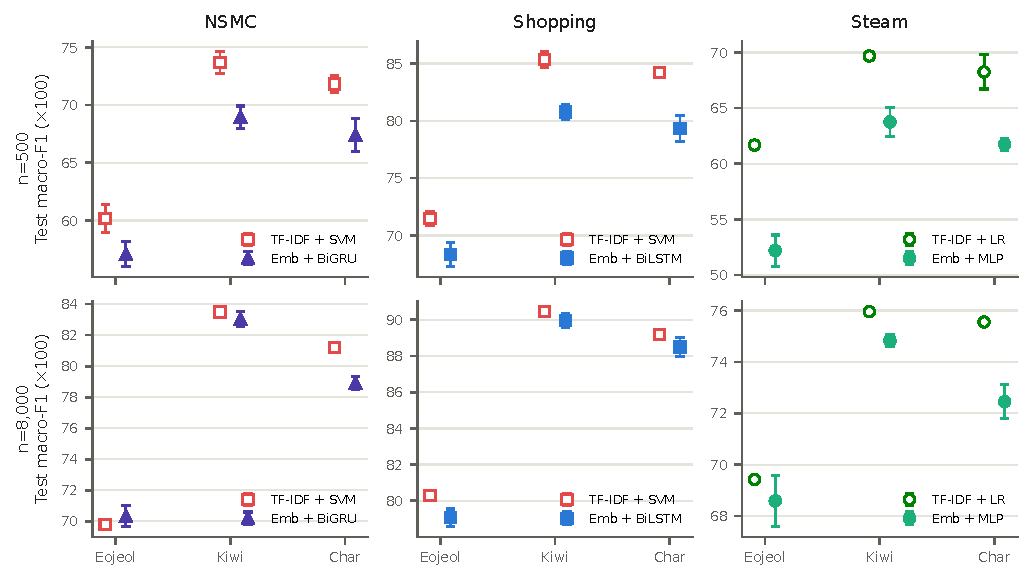
\includegraphics[width=\linewidth]{figures/fig5_tokenizers.pdf}
  \caption{Tokenizer effect: test macro-F1 of the best TF-IDF (hollow) and best neural
  (filled) method per dataset at $n=500$ (top) and $n=8{,}000$ (bottom); error bars are
  $\pm1$ std over \nSeeds{} seeds (sample std).}
  \label{fig:tokenizers}
\end{figure}

With each family using its best tokenizer, the neural $-$ TF-IDF gap is \ablationGapSmallNSMC{}
(NSMC), \ablationGapSmallShopping{} (Shopping) and \ablationGapSmallSteam{} (Steam) points
at $n=500$, and \ablationGapLargeNSMC, \ablationGapLargeShopping{} and
\ablationGapLargeSteam{} points at $n=8{,}000$ (\cref{tab:ablation,fig:tokenizers}). The best
TF-IDF tokenizer at 8{,}000 is \bestTokenizerTfidfNSMC/\bestTokenizerTfidfShopping/\bestTokenizerTfidfSteam{}
and the best neural tokenizer \bestTokenizerNeuralNSMC/\bestTokenizerNeuralShopping/\bestTokenizerNeuralSteam{}
(NSMC/Shopping/Steam). The main conclusion (whether the gap reaches \crossoverMargin{} point)
holds with the best tokenizers on NSMC: \ablationHoldsNSMC; Shopping: \ablationHoldsShopping;
Steam: \ablationHoldsSteam.

A stronger TF-IDF representation does not change the picture, because character $n$-grams
are \emph{not} stronger here. Kiwi morphemes are the best tokenizer for both families in
almost every cell of \cref{tab:ablation}, and eojeol tokens are clearly the worst. Korean
attaches particles and endings to the stem, so whole eojeol are sparse and most of them
are unseen at small sizes. The single exception is Shopping at $n=8{,}000$. There,
validation selects character $n$-grams for TF-IDF, but on test they do worse than Kiwi
morphemes. The paired gap with each family's validation-selected tokenizer therefore turns
positive (\ablationGapLargeShopping{} points). It still stays below the
\crossoverMargin-point margin, and it comes from a selection miss on the TF-IDF side, not
from a neural gain. Kiwi's linguistic knowledge helps both families. Removing it (eojeol or
characters) costs the TF-IDF and the neural model similar amounts, with no consistent
advantage for either. The conclusion of the main experiment (no crossover up to 8{,}000) is therefore not
an artefact of the tokenizer choice.

\section{Discussion}

\paragraph{How does model behavior change with scale?}
All families improve with more labels, but TF-IDF reaches useful performance earlier. Learned-from-scratch neural models close the gap near the upper end of each schedule. NSMC is the only domain where the neural advantage reaches and sustains the prespecified one-point margin. Shopping's best neural pipeline wins at full data without clearing the margin; Steam's top three neural methods are tightly grouped and also remain below it.

\paragraph{Does the improvement justify cost?}
There is no universal answer. Linear TF-IDF is fast, compact, and competitive at every tested scale. On NSMC, a team that values roughly \Result{story_full_gap_nsmc} additional macro-F1 points may accept \Result{story_fit_ratio_nsmc} times the fit time. On Shopping and Steam, the smaller gains make that trade harder to justify unless predictive quality dominates deployment constraints. Random Forest is rarely attractive because its sparse-text latency and model size are high without a matching quality gain.

\paragraph{What transfers across domains?}
The shared result is that pooling existing source labels substantially improves a low-label target-only Transformer. The domain-specific result is whether that pooled model beats TF-IDF and whether a contrastive loss helps. Shopping remains especially favorable to TF-IDF at low target budgets. Standard SupCon and DB-CDSupCon each win selected cells, but neither dominates pooled CE across targets and sizes.

\paragraph{Does DB-CDSupCon improve representations?}
The separation diagnostic changes in the intended direction only on Shopping when averaged across target sizes. NSMC and Steam move slightly downward. Even where separation rises, target macro-F1 does not rise at every size. A representation diagnostic is supporting evidence, not a substitute for the task metric.

\paragraph{Practical recommendations.}
With hundreds or a few thousand labels, start with TF-IDF plus a linear classifier. At tens of thousands of labels, compare that baseline with a small Transformer or gated RNN using the target hardware. If labeled source domains already exist, pooled CE is the essential transfer baseline. Add a contrastive objective only after a matched pooled comparison shows a stable benefit for the target domain.

\section{Limitations and threats to validity}

Ratings and recommendation flags are noisy proxies for sentiment. The benchmark covers three Korean review domains and binary labels, so the findings may not transfer to other genres, label schemes, or languages. NSMC uses an official test file while Shopping and Steam use seeded random splits.

All neural representations are learned from scratch. This isolates data scaling but does not answer how a pretrained Korean language model would behave. Each dataset-model pair receives the same number of tuning candidates, not the same compute budget, and selection occurs at 8,000 labels. A configuration that is optimal at that size may not be optimal at 200 labels or full data.

Three final seeds describe variation but provide little power for formal tests. We therefore report effect sizes, sample SDs, and raw paired seed differences without significance language. CUDA training and CPU classical timing reflect a practical mixed-device setup. They do not isolate architecture from hardware. PyTorch deterministic mode emitted a warning for one attention kernel, so the process is seeded and repeatable at the protocol level but is not claimed to be bitwise deterministic.

The bonus adds 4,000 source examples, uses one Transformer backbone, and evaluates only four target sizes. It tests whether existing source labels help, not whether source labeling is cost-free or whether total annotation decreases. Projection diagnostics use fixed deterministic samples and cosine pairs, but stored embeddings were not retained for alternative projections.

\section{Conclusion}
\label{sec:conclusion}

We measured when neural sequence models trained from scratch overtake TF-IDF
classifiers on Korean review sentiment. The crossover thresholds are
\crossoverNSMC{} (NSMC), \crossoverShopping{} (Shopping) and \crossoverSteam{} (Steam).
\TBD{final recommendation in two sentences}

\paragraph{Reproducibility.}
All code, configurations, per-run results and the scripts that regenerate every table,
figure and number in this report are in the \texttt{source/} folder
(\texttt{bash scripts/run\_everything.sh}).


\bibliographystyle{plainnat}
\bibliography{references}

\clearpage
\appendix
\section{Audit and completeness}
\begin{table}[t]
\centering
\caption{Result completeness. Smoke records are unplanned diagnostics and are excluded.}
\label{tab:completeness}
\small
\begin{tabular}{lrr}
\toprule
Phase & Completed & Expected \\
\midrule
Part 1 tuning & 270 & 270 \\
Part 1 final & 837 & 837 \\
Bonus tuning & 36 & 36 \\
Bonus final & 108 & 108 \\
\midrule
Total & 1,251 & 1,251 \\
\bottomrule
\end{tabular}
\end{table}


The audit outcome is \texttt{complete\_with\_declared\_exceptions}. All planned runs are complete. The declared exception concerns only the original derived bonus TF-IDF reference; the reporting rebuild fixes the selection rule from intact Part~1 atomic records.

\section{Additional result checks}
\begin{table*}[t]
\centering
\caption{Bonus target-domain macro-F1 (percentage points), mean $\pm$ sample SD ($n=3$). The TF-IDF and target-only Transformer rows reuse Part 1 runs.}
\label{tab:bonus-performance}
\scriptsize
\setlength{\tabcolsep}{3.5pt}
\begin{tabular}{llrrrr}
\toprule
Target & Method & 200 & 500 & 1,000 & 2,000 \\
\midrule
NSMC & Best TF-IDF & 60.62 $\pm$ 0.96 (3) & 63.99 $\pm$ 0.58 (3) & 67.02 $\pm$ 0.28 (3) & 69.65 $\pm$ 0.19 (3) \\
 & Target-only Transformer & 50.77 $\pm$ 3.52 (3) & 51.26 $\pm$ 6.13 (3) & 54.72 $\pm$ 5.97 (3) & 57.90 $\pm$ 1.17 (3) \\
 & Pooled CE & 62.82 $\pm$ 0.83 (3) & 64.73 $\pm$ 1.33 (3) & 66.55 $\pm$ 1.07 (3) & 68.71 $\pm$ 0.38 (3) \\
 & SupCon & 63.08 $\pm$ 0.79 (3) & 64.83 $\pm$ 1.32 (3) & 66.02 $\pm$ 1.80 (3) & 68.52 $\pm$ 0.68 (3) \\
 & DB-CDSupCon & 63.59 $\pm$ 0.75 (3) & 65.36 $\pm$ 0.34 (3) & 66.53 $\pm$ 0.74 (3) & 68.78 $\pm$ 0.62 (3) \\
\addlinespace
Shopping & Best TF-IDF & 71.93 $\pm$ 0.96 (3) & 76.73 $\pm$ 1.52 (3) & 79.81 $\pm$ 0.44 (3) & 81.86 $\pm$ 0.31 (3) \\
 & Target-only Transformer & 63.92 $\pm$ 2.74 (3) & 64.70 $\pm$ 5.53 (3) & 72.51 $\pm$ 2.31 (3) & 71.75 $\pm$ 7.66 (3) \\
 & Pooled CE & 69.11 $\pm$ 3.29 (3) & 74.02 $\pm$ 0.67 (3) & 75.86 $\pm$ 1.58 (3) & 75.45 $\pm$ 2.19 (3) \\
 & SupCon & 69.48 $\pm$ 3.63 (3) & 74.22 $\pm$ 0.85 (3) & 75.52 $\pm$ 1.70 (3) & 78.04 $\pm$ 0.70 (3) \\
 & DB-CDSupCon & 69.73 $\pm$ 3.77 (3) & 74.30 $\pm$ 0.46 (3) & 75.35 $\pm$ 1.70 (3) & 77.88 $\pm$ 0.69 (3) \\
\addlinespace
Steam & Best TF-IDF & 60.50 $\pm$ 0.60 (3) & 62.42 $\pm$ 0.58 (3) & 64.49 $\pm$ 0.46 (3) & 67.32 $\pm$ 0.44 (3) \\
 & Target-only Transformer & 49.18 $\pm$ 2.60 (3) & 54.20 $\pm$ 1.14 (3) & 58.02 $\pm$ 1.87 (3) & 57.33 $\pm$ 5.48 (3) \\
 & Pooled CE & 62.71 $\pm$ 1.04 (3) & 62.83 $\pm$ 1.33 (3) & 65.18 $\pm$ 0.35 (3) & 66.29 $\pm$ 0.41 (3) \\
 & SupCon & 61.70 $\pm$ 0.20 (3) & 63.93 $\pm$ 0.14 (3) & 64.67 $\pm$ 0.57 (3) & 66.51 $\pm$ 0.97 (3) \\
 & DB-CDSupCon & 62.78 $\pm$ 1.50 (3) & 62.83 $\pm$ 0.92 (3) & 64.97 $\pm$ 0.84 (3) & 66.14 $\pm$ 0.66 (3) \\
\addlinespace
\bottomrule
\end{tabular}
\end{table*}

\begin{table}[t]
\centering
\caption{Bonus label-efficiency result. Crossovers compare each method with the fixed best Part 1 TF-IDF reference at the same target size. Savings are reported only if both the method and target-only Transformer crossovers are observed.}
\label{tab:bonus-labels}
\scriptsize
\resizebox{\columnwidth}{!}{%
\begin{tabular}{@{}llrr@{}}
\toprule
Target & Method & Crossover & Labels saved \\
\midrule
NSMC & Target-only Transformer & Not observed & Not estimable \\
 & Pooled CE & 200 & Not estimable \\
 & SupCon & 200 & Not estimable \\
 & DB-CDSupCon & 200 & Not estimable \\
\addlinespace
Shopping & Target-only Transformer & Not observed & Not estimable \\
 & Pooled CE & Not observed & Not estimable \\
 & SupCon & Not observed & Not estimable \\
 & DB-CDSupCon & Not observed & Not estimable \\
\addlinespace
Steam & Target-only Transformer & Not observed & Not estimable \\
 & Pooled CE & 200 & Not estimable \\
 & SupCon & 200 & Not estimable \\
 & DB-CDSupCon & 200 & Not estimable \\
\addlinespace
\bottomrule
\end{tabular}
}
\end{table}

\begin{table}[t]
\centering
\caption{Bonus source retention and representation separation, averaged over the four target-label sizes. Retention is the source macro-F1 difference from pooled CE.}
\label{tab:bonus-diagnostics}
\scriptsize
\begin{tabular}{llrr}
\toprule
Target & Method & Source $\Delta$ & Separation gap \\
\midrule
NSMC & Pooled CE & +0.000 & 0.095 \\
 & SupCon & -0.000 & 0.094 \\
 & DB-CDSupCon & +0.005 & 0.088 \\
\addlinespace
Shopping & Pooled CE & +0.000 & 0.078 \\
 & SupCon & +0.015 & 0.091 \\
 & DB-CDSupCon & +0.015 & 0.086 \\
\addlinespace
Steam & Pooled CE & +0.000 & 0.154 \\
 & SupCon & -0.001 & 0.146 \\
 & DB-CDSupCon & -0.001 & 0.147 \\
\addlinespace
\bottomrule
\end{tabular}
\end{table}


\begin{figure}[ht]
  \centering
  \includegraphics[width=0.62\textwidth]{confusion_comparison.pdf}
  \caption{NSMC full-data confusion matrices summed over three seeds and normalized within the actual class. Parentheses give summed counts.}
  \label{fig:confusion}
\end{figure}

\section{Frozen configurations}
\begin{longtable}{lll >{\raggedright\arraybackslash}p{7.2cm}}
\caption{Frozen Part 1 configurations selected at 8,000 labels with tuning seed 777.}\label{tab:selected-configs}\\
\toprule
Dataset & Model & ID & Configuration \\
\midrule
\endfirsthead
\toprule
Dataset & Model & ID & Configuration \\
\midrule
\endhead
NSMC & TF-IDF + LR & lr06 & \texttt{\{"C": 2.0, "id": "lr06", "max\_iter": 3000, "solver": "liblinear"\}} \\
NSMC & TF-IDF + SVM & svm05 & \texttt{\{"C": 0.25, "id": "svm05"\}} \\
NSMC & TF-IDF + RF & rf09 & \texttt{\{"id": "rf09", "max\_depth": null, "max\_features": "sqrt", "min\_samples\_leaf": 2, "n\_estimators": 700\}} \\
NSMC & TF-IDF + XGBoost & xgb03 & \texttt{\{"colsample\_bytree": 0.8, "id": "xgb03", "learning\_rate": 0.05, "max\_depth": 4, "n\_estimators": 400, "reg\_lambda": 1.0, "subsample": 0.8\}} \\
NSMC & Avg. embeddings + MLP & mlp08 & \texttt{\{"dropout": 0.3, "embedding\_dim": 128, "hidden\_dim": 288, "id": "mlp08", "learning\_rate": 0.002, "num\_layers": 2\}} \\
NSMC & LSTM & lstm08 & \texttt{\{"dropout": 0.3, "embedding\_dim": 128, "hidden\_dim": 112, "id": "lstm08", "learning\_rate": 0.002, "num\_layers": 2\}} \\
NSMC & GRU & gru08 & \texttt{\{"dropout": 0.3, "embedding\_dim": 128, "hidden\_dim": 128, "id": "gru08", "learning\_rate": 0.002, "num\_layers": 2\}} \\
NSMC & Transformer & tr07 & \texttt{\{"dropout": 0.4, "embedding\_dim": 128, "ff\_multiplier": 2, "hidden\_dim": 128, "id": "tr07", "learning\_rate": 0.001, "num\_heads": 4, "num\_layers": 2\}} \\
NSMC & Mamba & mb08 & \texttt{\{"d\_conv": 4, "d\_state": 16, "dropout": 0.3, "embedding\_dim": 128, "expand": 2, "hidden\_dim": 128, "id": "mb08", "learning\_rate": 0.002, "num\_layers": 2\}} \\
Shopping & TF-IDF + LR & lr06 & \texttt{\{"C": 2.0, "id": "lr06", "max\_iter": 3000, "solver": "liblinear"\}} \\
Shopping & TF-IDF + SVM & svm05 & \texttt{\{"C": 0.25, "id": "svm05"\}} \\
Shopping & TF-IDF + RF & rf09 & \texttt{\{"id": "rf09", "max\_depth": null, "max\_features": "sqrt", "min\_samples\_leaf": 2, "n\_estimators": 700\}} \\
Shopping & TF-IDF + XGBoost & xgb03 & \texttt{\{"colsample\_bytree": 0.8, "id": "xgb03", "learning\_rate": 0.05, "max\_depth": 4, "n\_estimators": 400, "reg\_lambda": 1.0, "subsample": 0.8\}} \\
Shopping & Avg. embeddings + MLP & mlp08 & \texttt{\{"dropout": 0.3, "embedding\_dim": 128, "hidden\_dim": 288, "id": "mlp08", "learning\_rate": 0.002, "num\_layers": 2\}} \\
Shopping & LSTM & lstm04 & \texttt{\{"dropout": 0.2, "embedding\_dim": 96, "hidden\_dim": 96, "id": "lstm04", "learning\_rate": 0.002, "num\_layers": 1\}} \\
Shopping & GRU & gru08 & \texttt{\{"dropout": 0.3, "embedding\_dim": 128, "hidden\_dim": 128, "id": "gru08", "learning\_rate": 0.002, "num\_layers": 2\}} \\
Shopping & Transformer & tr07 & \texttt{\{"dropout": 0.4, "embedding\_dim": 128, "ff\_multiplier": 2, "hidden\_dim": 128, "id": "tr07", "learning\_rate": 0.001, "num\_heads": 4, "num\_layers": 2\}} \\
Shopping & Mamba & mb08 & \texttt{\{"d\_conv": 4, "d\_state": 16, "dropout": 0.3, "embedding\_dim": 128, "expand": 2, "hidden\_dim": 128, "id": "mb08", "learning\_rate": 0.002, "num\_layers": 2\}} \\
Steam & TF-IDF + LR & lr06 & \texttt{\{"C": 2.0, "id": "lr06", "max\_iter": 3000, "solver": "liblinear"\}} \\
Steam & TF-IDF + SVM & svm05 & \texttt{\{"C": 0.25, "id": "svm05"\}} \\
Steam & TF-IDF + RF & rf09 & \texttt{\{"id": "rf09", "max\_depth": null, "max\_features": "sqrt", "min\_samples\_leaf": 2, "n\_estimators": 700\}} \\
Steam & TF-IDF + XGBoost & xgb03 & \texttt{\{"colsample\_bytree": 0.8, "id": "xgb03", "learning\_rate": 0.05, "max\_depth": 4, "n\_estimators": 400, "reg\_lambda": 1.0, "subsample": 0.8\}} \\
Steam & Avg. embeddings + MLP & mlp08 & \texttt{\{"dropout": 0.3, "embedding\_dim": 128, "hidden\_dim": 288, "id": "mlp08", "learning\_rate": 0.002, "num\_layers": 2\}} \\
Steam & LSTM & lstm08 & \texttt{\{"dropout": 0.3, "embedding\_dim": 128, "hidden\_dim": 112, "id": "lstm08", "learning\_rate": 0.002, "num\_layers": 2\}} \\
Steam & GRU & gru08 & \texttt{\{"dropout": 0.3, "embedding\_dim": 128, "hidden\_dim": 128, "id": "gru08", "learning\_rate": 0.002, "num\_layers": 2\}} \\
Steam & Transformer & tr08 & \texttt{\{"dropout": 0.3, "embedding\_dim": 128, "ff\_multiplier": 2, "hidden\_dim": 128, "id": "tr08", "learning\_rate": 0.002, "num\_heads": 8, "num\_layers": 2\}} \\
Steam & Mamba & mb07 & \texttt{\{"d\_conv": 3, "d\_state": 16, "dropout": 0.4, "embedding\_dim": 128, "expand": 2, "hidden\_dim": 128, "id": "mb07", "learning\_rate": 0.001, "num\_layers": 2\}} \\
\bottomrule
\end{longtable}


\section{Additional interpretation details}

The machine-readable appendix is more exhaustive than a printed table. \texttt{part1\_metrics\_by\_seed.csv} contains all 837 Part~1 final rows. \texttt{part1\_summary.csv} contains every learning-curve cell, gains from the previous and approximate half-size budgets, and normalized log-size AULC. \texttt{bonus\_metrics\_by\_seed\_corrected.csv} contains all five bonus comparison methods with corrected TF-IDF reuse. \texttt{bonus\_paired\_differences.csv} records every ordered paired seed difference. Cost, source-retention, representation, and label-efficiency files sit beside them.

\paragraph{Loss and deployment.} The SupCon projection is a linear layer, ReLU, second linear layer, and L2 normalization. It adds \Result{bonus_projection_parameters} trainable parameters during SupCon training. The deployed classifier bypasses this head, leaving \Result{bonus_deployed_parameters} parameters for pooled CE, SupCon, and DB-CDSupCon. Thus contrastive training changes fit time and peak training memory but not the deployed computation graph.

\end{document}
